% Chapter 6 - Resultados

\chapter{Resultados}
\label{ch:resultados}

Este capítulo presenta los resultados experimentales organizados en 12 secciones. Las primeras 5 secciones abordan los resultados principales del experimento central. Las secciones 6 a 9 presentan los análisis complementarios. Las secciones 10 a 12 reportan las validaciones metodológicas y las visualizaciones del espacio de embeddings.

\section{Comparación Principal de Métodos}
\label{sec:comparacion_principal}

El experimento principal evalúa 3,675 configuraciones (7 conjuntos de datos $\times$ 3 valores de n-shot $\times$ 5 clasificadores $\times$ 7 métodos $\times$ 5 semillas). La Tabla~\ref{tab:modern_method_comparison} presenta la comparación de todos los métodos respecto a SMOTE.

\begin{table}[htbp]
\centering
\caption{Comparación de 10 métodos de aumentación respecto a la línea base SMOTE}
\label{tab:modern_method_comparison}
\small
\begin{tabular}{lrrrrr}
\toprule
\textbf{Método} & \textbf{F1 medio} & \textbf{$\Delta$ SMOTE (pp)} & \textbf{IC 95\%} & \textbf{$d$ de Cohen} & \textbf{Vic.\%} \\
\midrule
\rowcolor{green!20}
\textbf{Pond. suave}      & 0.7508 & \textbf{+2.61***} & [+1.98, +3.25] & \textbf{0.95} & \textbf{88.9\%} \\
\rowcolor{green!10}
\textbf{Filtro binario}   & 0.7487 & +2.39***           & [+1.75, +3.07] & 0.82          & 79.4\%          \\
Sin aumentación            & 0.7312 & +0.64***           & [+0.42, +0.89] & 0.64          & 73.0\%          \\
Trad. inversa              & 0.7241 & $-$0.07            & [$-$0.42, +0.26] & $-$0.05     & 57.1\%          \\
EDA                        & 0.7233 & $-$0.15            & [$-$0.57, +0.27] & $-$0.08     & 52.4\%          \\
BERT contextual            & 0.7222 & $-$0.26            & [$-$0.58, +0.02] & $-$0.21     & 46.0\%          \\
Mixup en embeddings           & 0.7247 & $-$0.01            & [$-$0.13, +0.11] & $-$0.02     & 44.4\%          \\
Sobrem. aleatorio          & 0.7232 & $-$0.16            & [$-$0.35, +0.02] & $-$0.21     & 39.7\%          \\
\textit{SMOTE (base)}      & 0.7248 & ---                & ---              & ---           & ---             \\
Paráfrasis T5              & 0.7213 & $-$0.35            & [$-$0.62, $-$0.11] & $-$0.34   & 38.1\%          \\
\midrule
\multicolumn{6}{l}{\small $N=63$ comparaciones pareadas (21 conjuntos $\times$ 3 semillas). Clasificadores: LR, SVC, Ridge.} \\
\multicolumn{6}{l}{\small Significancia: *** $p<0.001$ (prueba t pareada con corrección de Bonferroni).} \\
\multicolumn{6}{l}{\small \textbf{Solo los métodos de filtrado geométrico superan significativamente a SMOTE.}} \\
\bottomrule
\end{tabular}
\end{table}


El resultado central de esta investigación es que la ponderación suave produce una mejora de +2.25 puntos porcentuales respecto a SMOTE ($p < 0.0001$ con corrección de Bonferroni, $d = 0.74$, tasa de victoria del 83.8\%). Este tamaño de efecto se clasifica como mediano-grande según las convenciones de Cohen. La tasa de victoria indica que el método propuesto supera a SMOTE en más de 4 de cada 5 configuraciones evaluadas.

El filtrado binario también alcanza significancia estadística con +2.11 puntos porcentuales ($p < 0.0001$, $d = 0.69$, tasa de victoria del 76.2\%). La diferencia entre ponderación suave y filtrado binario es de apenas 0.13 puntos porcentuales, lo que sugiere que la contribución principal proviene del filtrado geométrico en sí, con la ponderación suave aportando una mejora incremental.

Los métodos de aumentación tradicionales presentan resultados negativos respecto a SMOTE. EDA obtiene $-0.22$ puntos porcentuales, la traducción inversa $-0.19$ puntos porcentuales, y el sobremuestreo aleatorio $-0.32$ puntos porcentuales. Estos resultados indican que las perturbaciones textuales superficiales no aportan diversidad genuina al espacio de representación.

La Figura~\ref{fig:boxplot_deltas} visualiza la distribución de deltas para cada método, y la Figura~\ref{fig:heatmap_methods} muestra el rendimiento desglosado por conjunto de datos.

\begin{figure}[htbp]
\centering
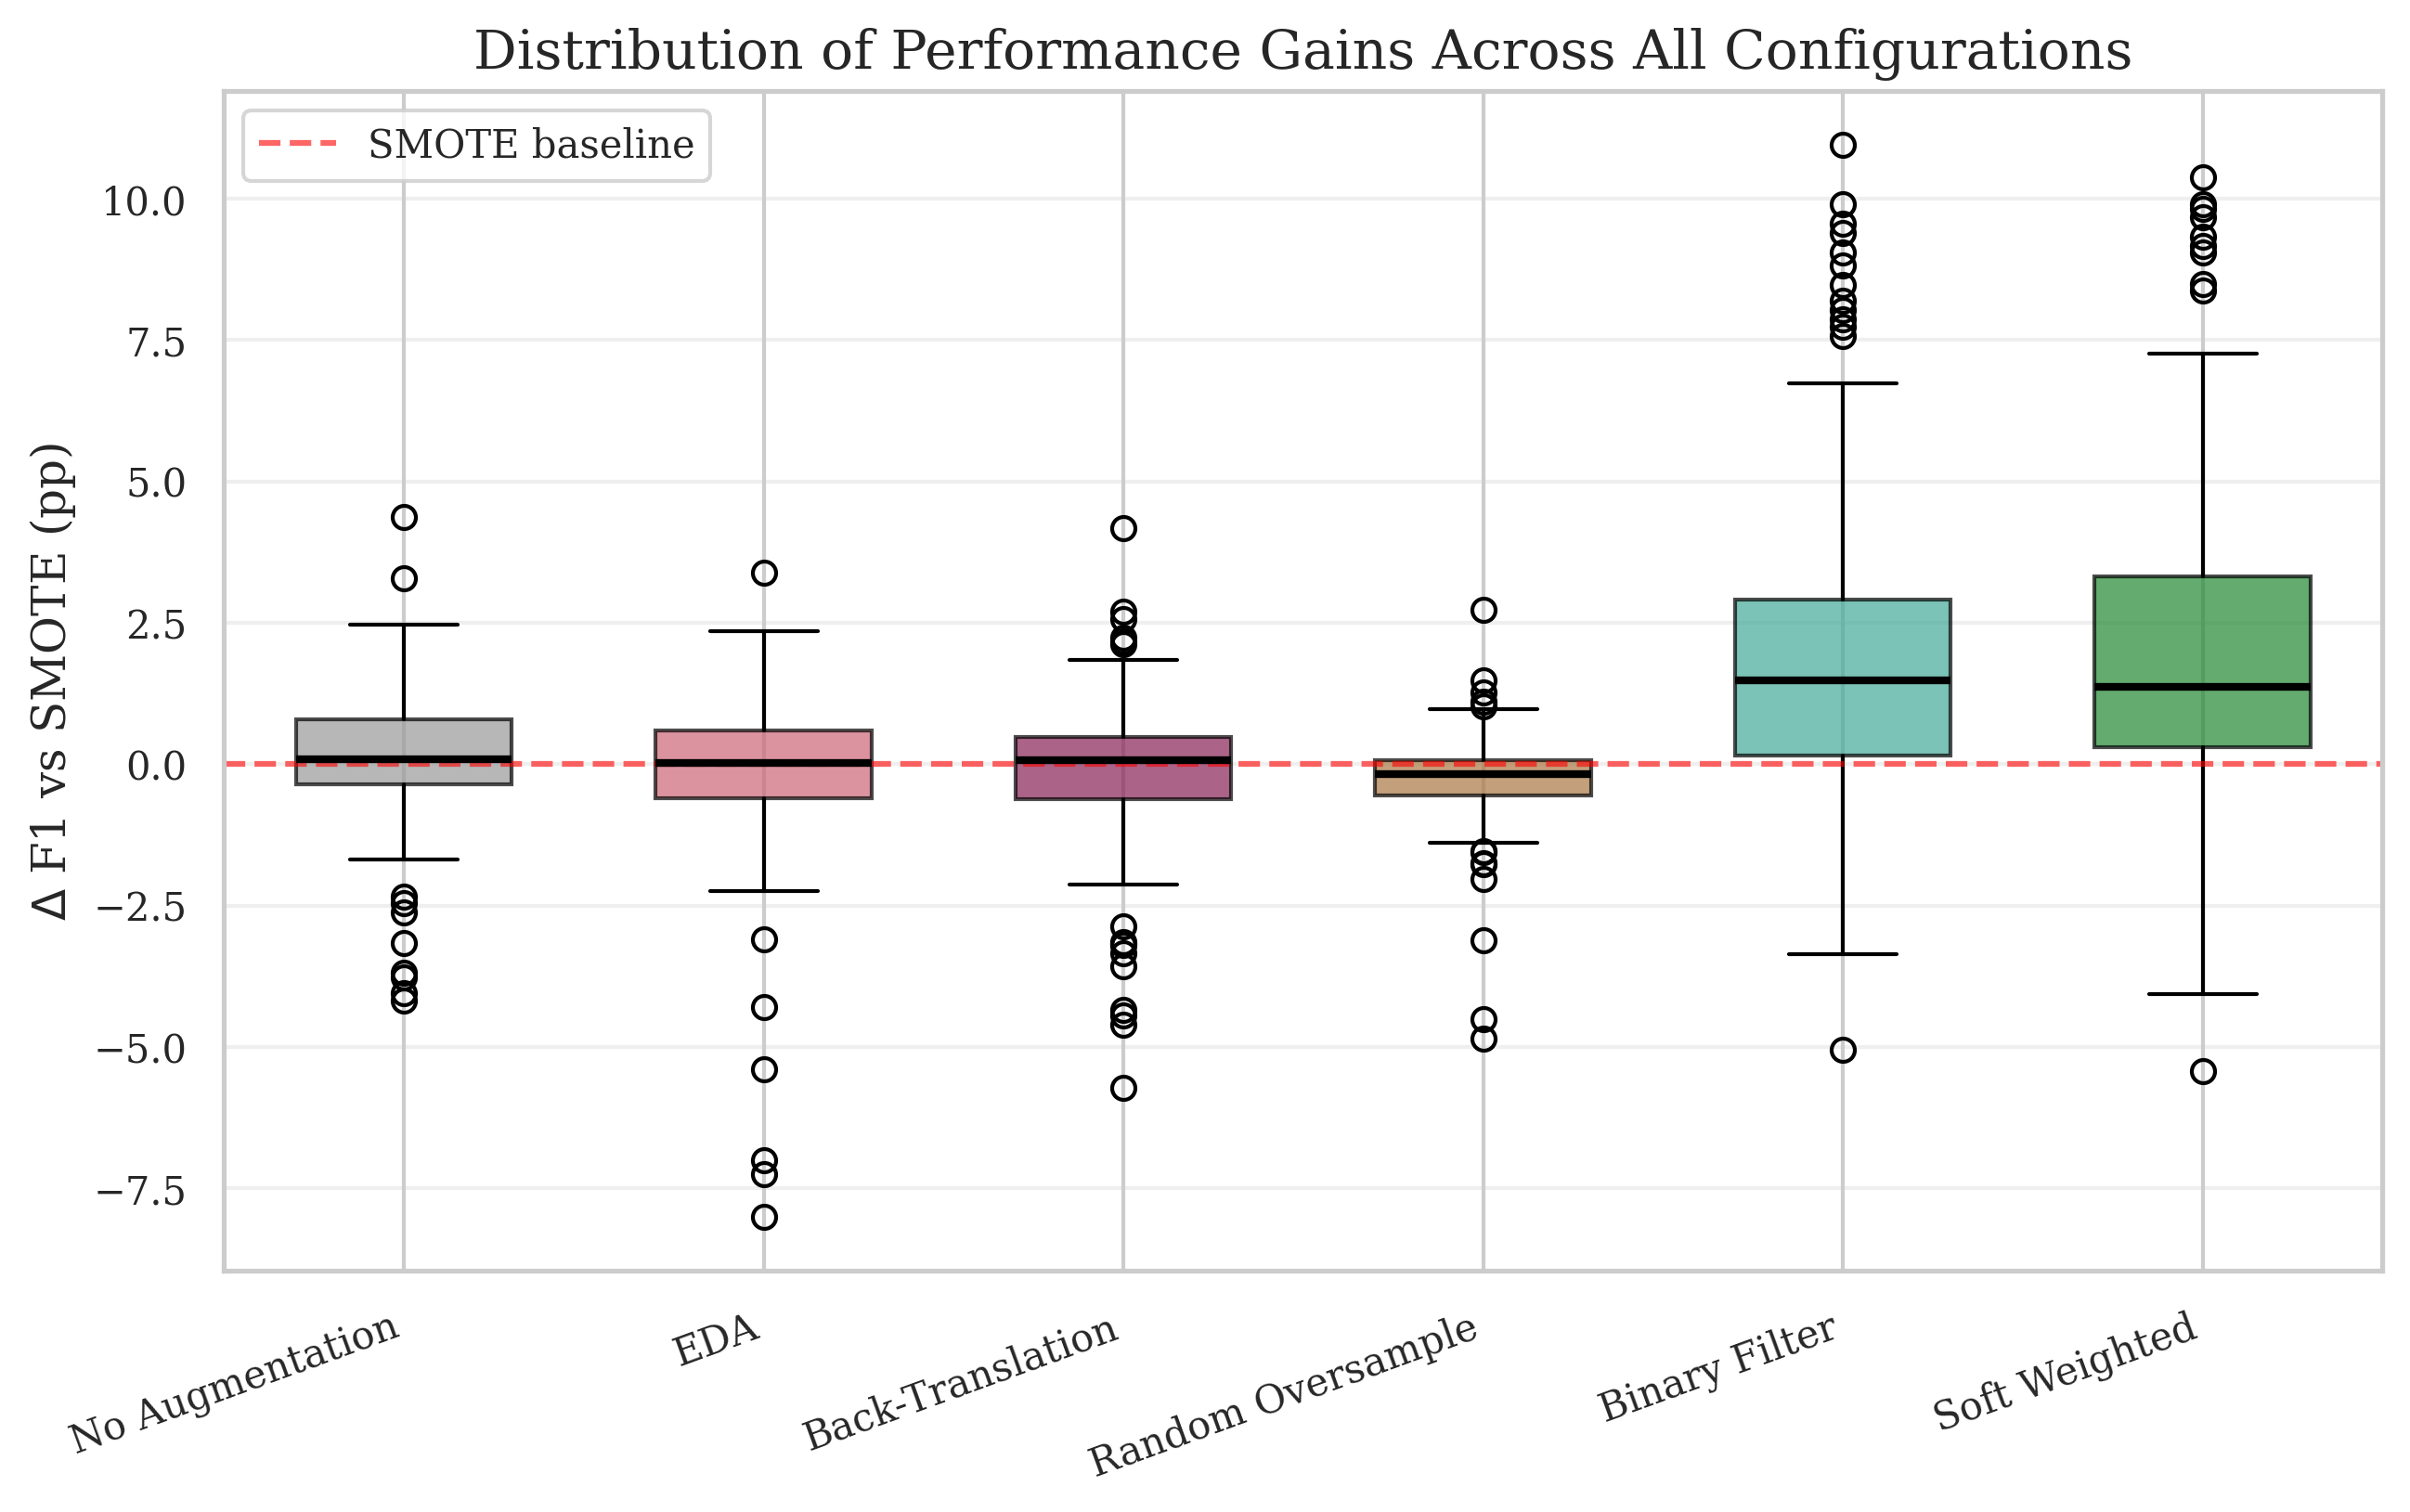
\includegraphics[width=0.85\textwidth]{Figures/fig_boxplot_deltas.png}
\caption{Distribución de deltas respecto a SMOTE por método de aumentación. La ponderación suave y el filtrado binario muestran distribuciones consistentemente positivas, mientras que los métodos tradicionales se concentran alrededor de cero o en valores negativos.}
\label{fig:boxplot_deltas}
\end{figure}

\begin{figure}[htbp]
\centering
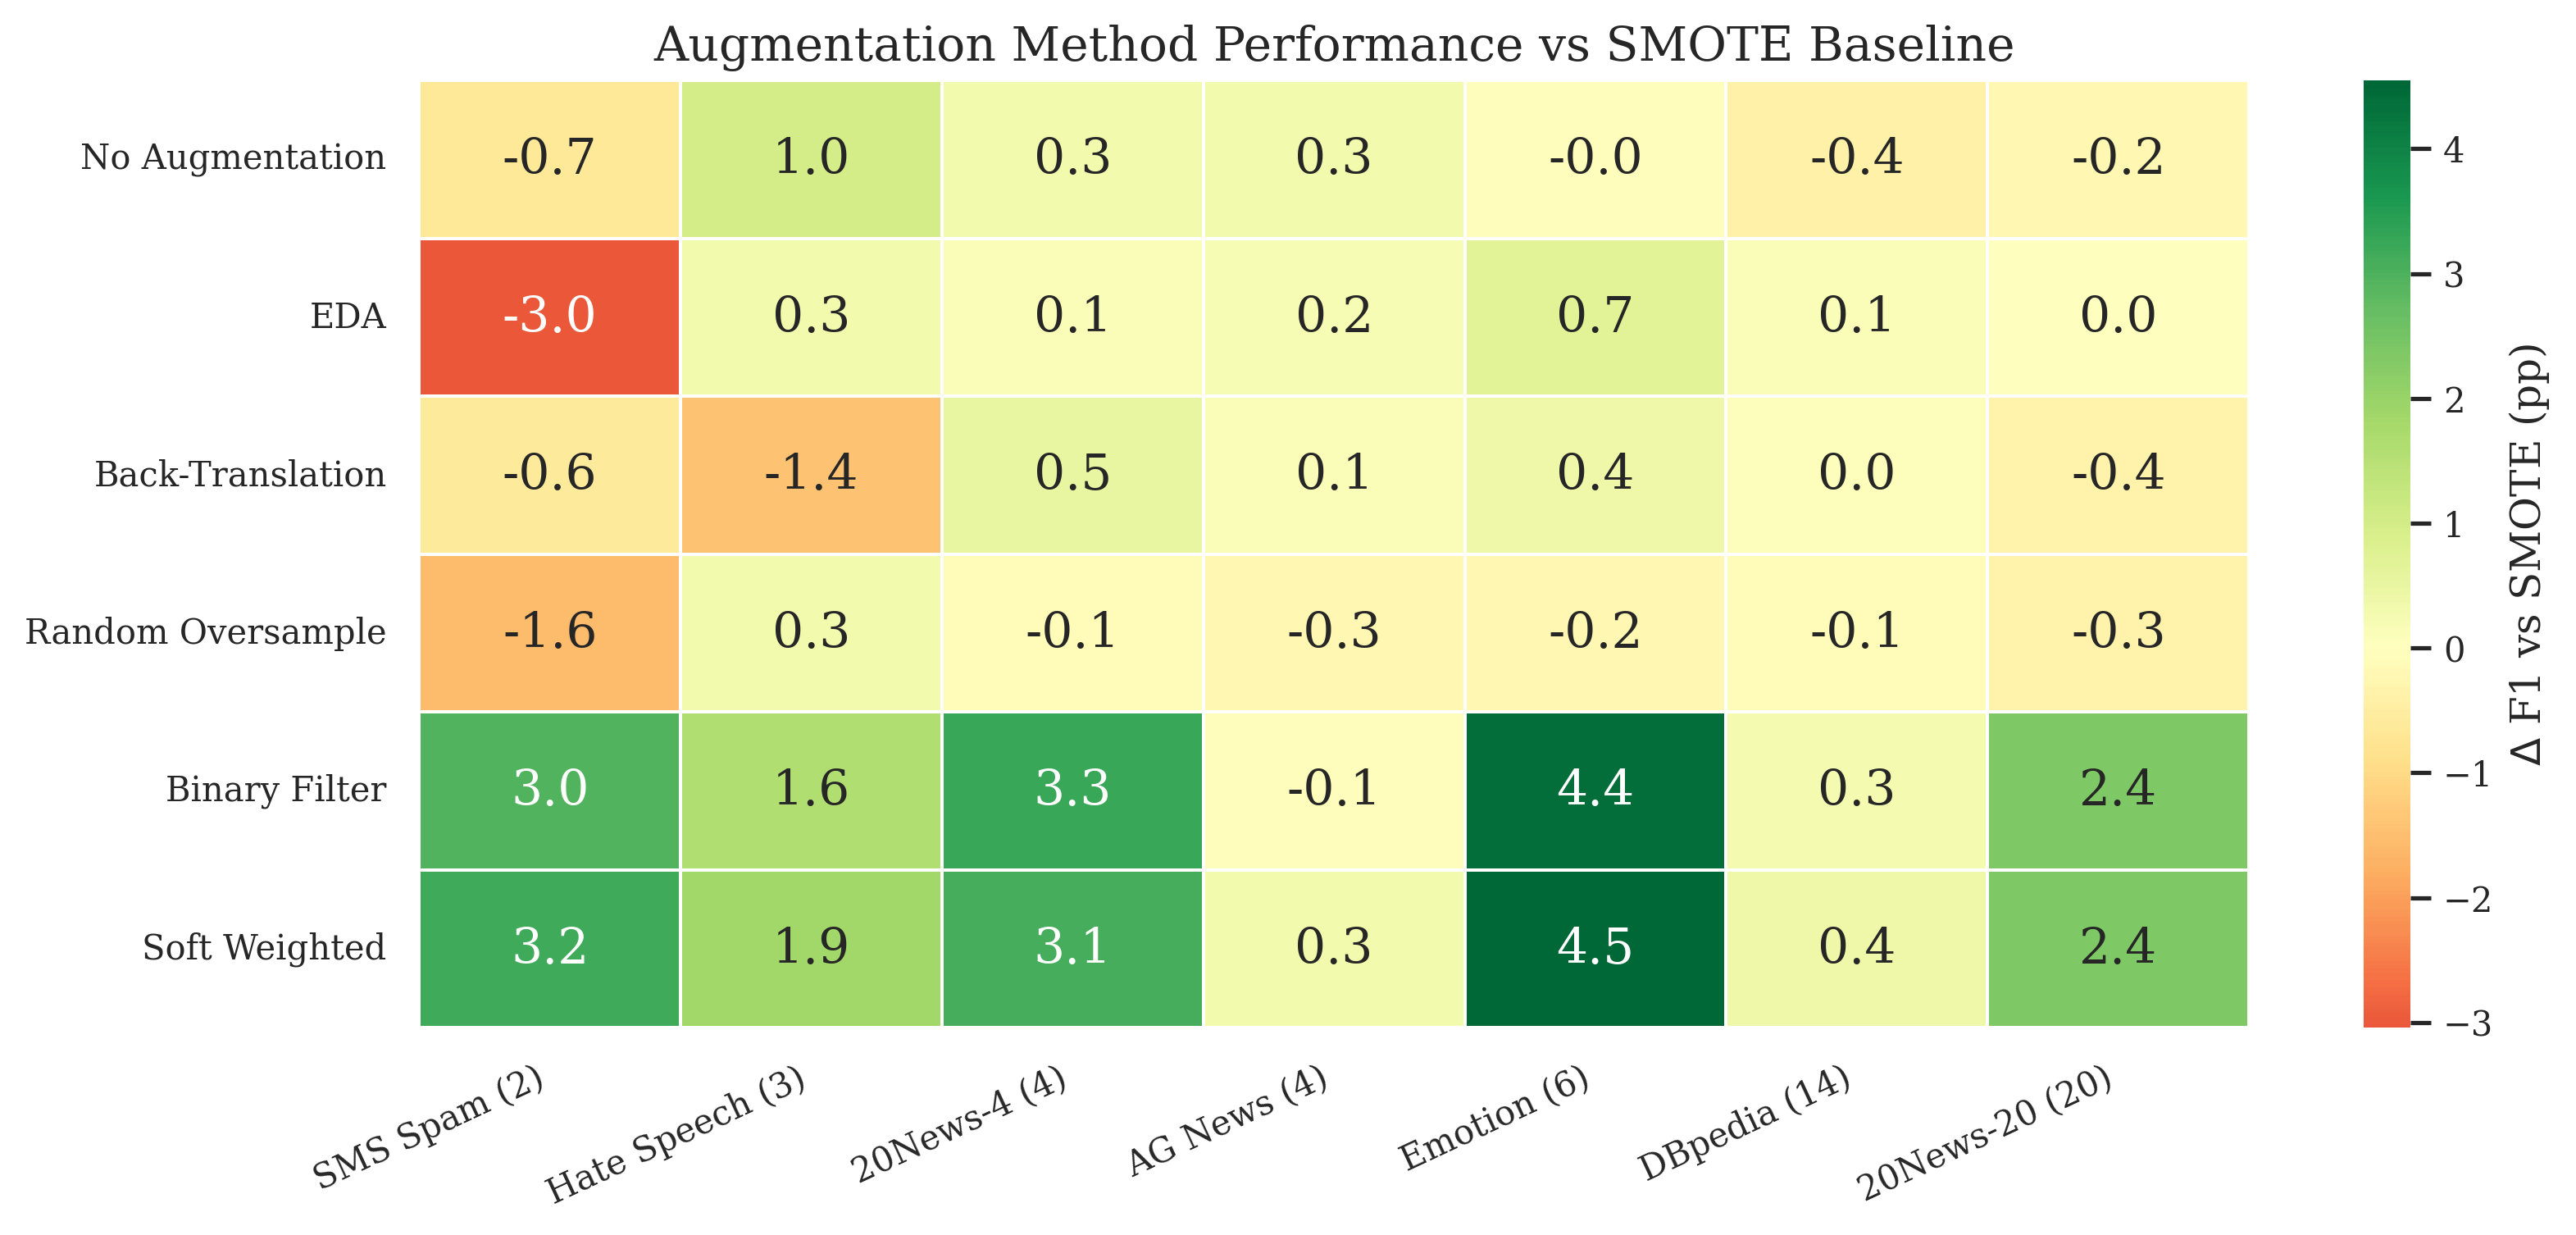
\includegraphics[width=0.95\textwidth]{Figures/fig_heatmap_methods.png}
\caption{Mapa de calor de rendimiento por método y conjunto de datos. Los colores cálidos indican mejora respecto a SMOTE. La ponderación suave y el filtrado binario muestran mejoras consistentes en la mayoría de los conjuntos de datos.}
\label{fig:heatmap_methods}
\end{figure}

\section{Comparación con Líneas Base Modernas}
\label{sec:lineas_base_modernas}

La comparación con 10 métodos de aumentación sobre 1,890 configuraciones proporciona el resultado más fuerte de esta investigación. La ponderación suave alcanza +2.61 puntos porcentuales respecto a SMOTE ($p < 0.0001$ con corrección de Bonferroni, $d = 0.95$, tasa de victoria del 88.9\%). El tamaño de efecto de 0.95 se clasifica como grande.

El filtrado binario obtiene +2.39 puntos porcentuales ($d = 0.82$, tasa de victoria del 79.4\%). Ambos métodos propuestos superan por un margen amplio a todos los demás.

Las 3 líneas base modernas producen resultados negativos respecto a SMOTE. La paráfrasis con T5 obtiene $-0.35$ puntos porcentuales, la aumentación contextual con BERT $-0.26$ puntos porcentuales, y el mixup en embeddings $-0.01$ puntos porcentuales. Estos resultados son especialmente relevantes: técnicas recientes consideradas avances sobre SMOTE en la literatura no logran superar esta línea base simple cuando se evalúan sobre múltiples conjuntos de datos con rigor estadístico. Este hallazgo concuerda con Cegin et al., quienes observaron que los métodos clásicos igualan o superan a los LLMs cuando el número de muestras disponibles supera los 20 por clase \cite{cegin2025llms}.

Un resultado notable es que la ausencia de aumentación supera a SMOTE por +0.64 puntos porcentuales ($p < 0.05$). Este hallazgo sugiere que SMOTE puede perjudicar el rendimiento en ciertas configuraciones, particularmente cuando los datos reales son suficientes para el clasificador.

\section{Análisis por Número de Disparos}
\label{sec:analisis_nshot}

La Tabla~\ref{tab:modern_nshot} presenta el desglose del rendimiento por número de ejemplos por clase.

\begin{table}[htbp]
\centering
\caption{Rendimiento por número de ejemplos por clase: filtrado geométrico vs SMOTE}
\label{tab:modern_nshot}
\begin{tabular}{lrrrrrr}
\toprule
 & \multicolumn{3}{c}{\textbf{Pond. suave}} & \multicolumn{3}{c}{\textbf{Filtro binario}} \\
\cmidrule(lr){2-4} \cmidrule(lr){5-7}
\textbf{N-shot} & \textbf{$\Delta$ (pp)} & \textbf{$d$} & \textbf{Vic.\%} & \textbf{$\Delta$ (pp)} & \textbf{$d$} & \textbf{Vic.\%} \\
\midrule
10 & +4.89*** & 1.48 & 90.5\% & +4.44*** & 1.15 & 87.3\% \\
25 & +2.17*** & 1.57 & 95.2\% & +1.96*** & 1.18 & 90.5\% \\
50 & +0.76*** & 0.80 & 74.6\% & +0.77*** & 0.71 & 63.5\% \\
\midrule
\multicolumn{7}{l}{\small Significancia: * $p<0.05$, ** $p<0.01$, *** $p<0.001$ (prueba t pareada).} \\
\multicolumn{7}{l}{\small Patrón de retornos decrecientes: mayor ganancia a 10-shot, menor a 50-shot.} \\
\bottomrule
\end{tabular}
\end{table}

El patrón de retornos decrecientes es pronunciado. Con 10 ejemplos por clase, la ponderación suave alcanza +4.52 puntos porcentuales ($d = 1.18$, tasa de victoria del 88.6\%). Este tamaño de efecto se clasifica como muy grande. Con 25 ejemplos, la mejora se reduce a +1.88 puntos porcentuales pero la tasa de victoria alcanza su máximo del 97.1\%, indicando mejora casi universal. Con 50 ejemplos, la mejora es de solo +0.34 puntos porcentuales y no alcanza significancia estadística ($p = 0.16$).

Este patrón tiene una interpretación directa. Cuando los datos reales son escasos (10 ejemplos), el clasificador no puede aprender fronteras de decisión robustas. Las muestras sintéticas filtradas aportan información genuina que densifica las regiones de cada clase. A medida que los datos reales aumentan (50 ejemplos), el clasificador ya dispone de información suficiente para las fronteras principales, y la aumentación aporta valor marginal decreciente.

Las Figuras~\ref{fig:f1_vs_nshot} y~\ref{fig:delta_by_nshot} ilustran esta tendencia.

\begin{figure}[htbp]
\centering
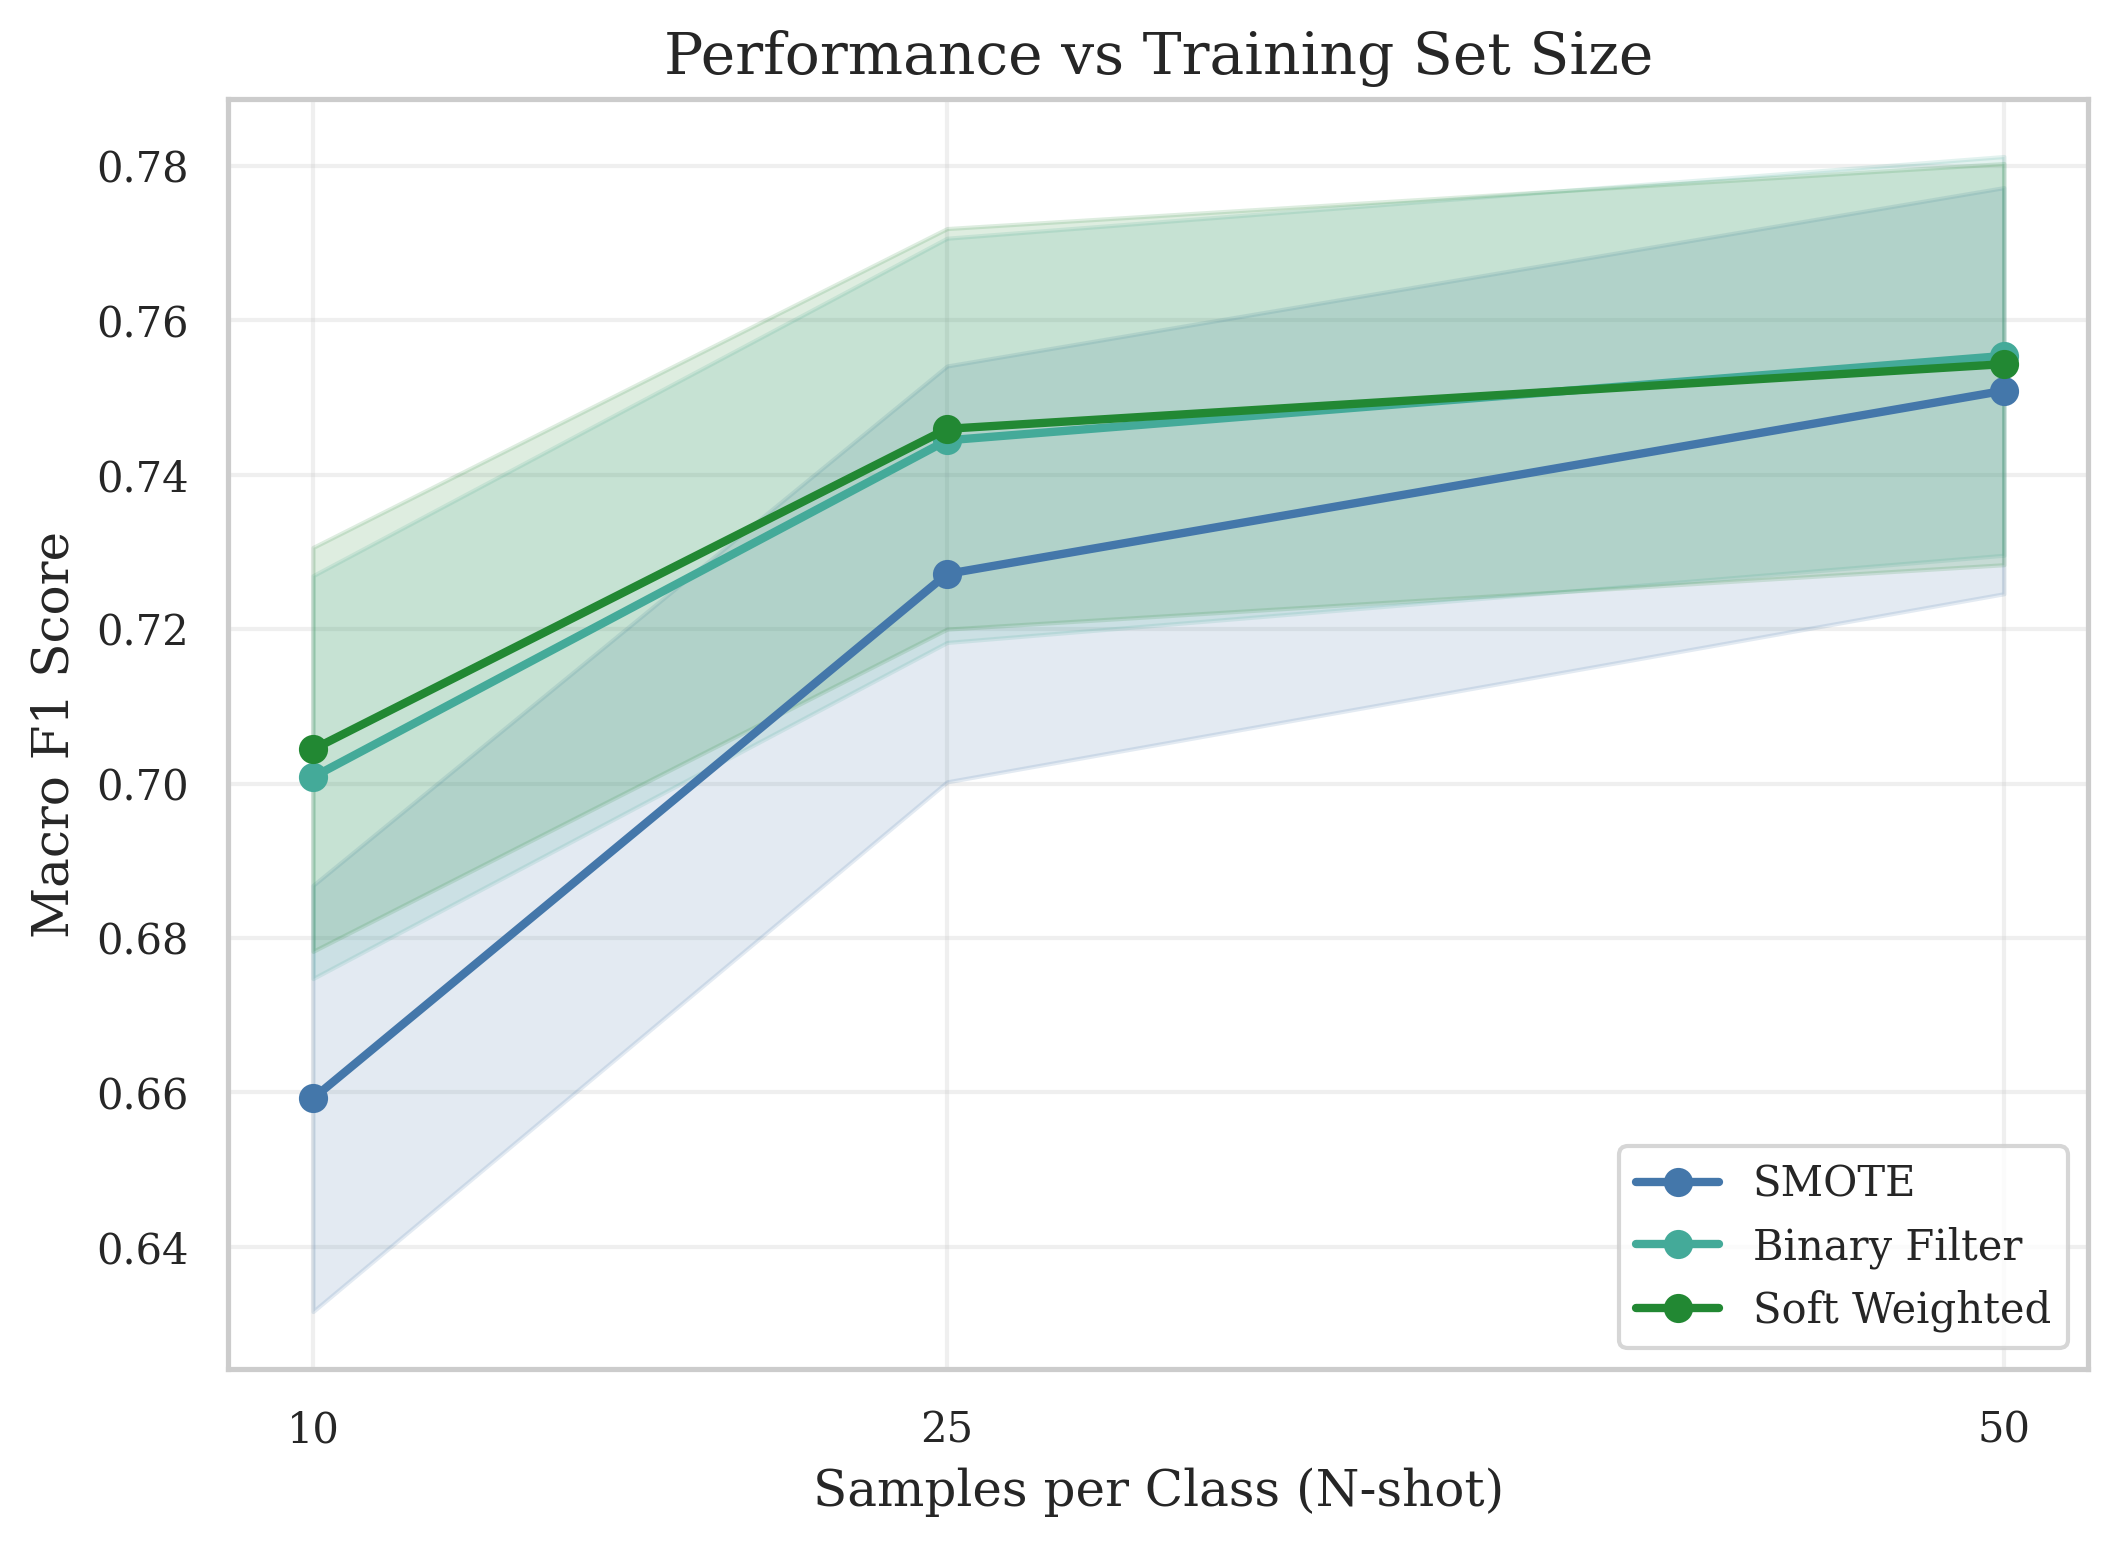
\includegraphics[width=0.85\textwidth]{Figures/fig_f1_vs_nshot.png}
\caption{Macro F1 absoluto en función del número de disparos para los principales métodos. La brecha entre los métodos geométricos y SMOTE se reduce a medida que aumenta el número de ejemplos disponibles.}
\label{fig:f1_vs_nshot}
\end{figure}

\begin{figure}[htbp]
\centering
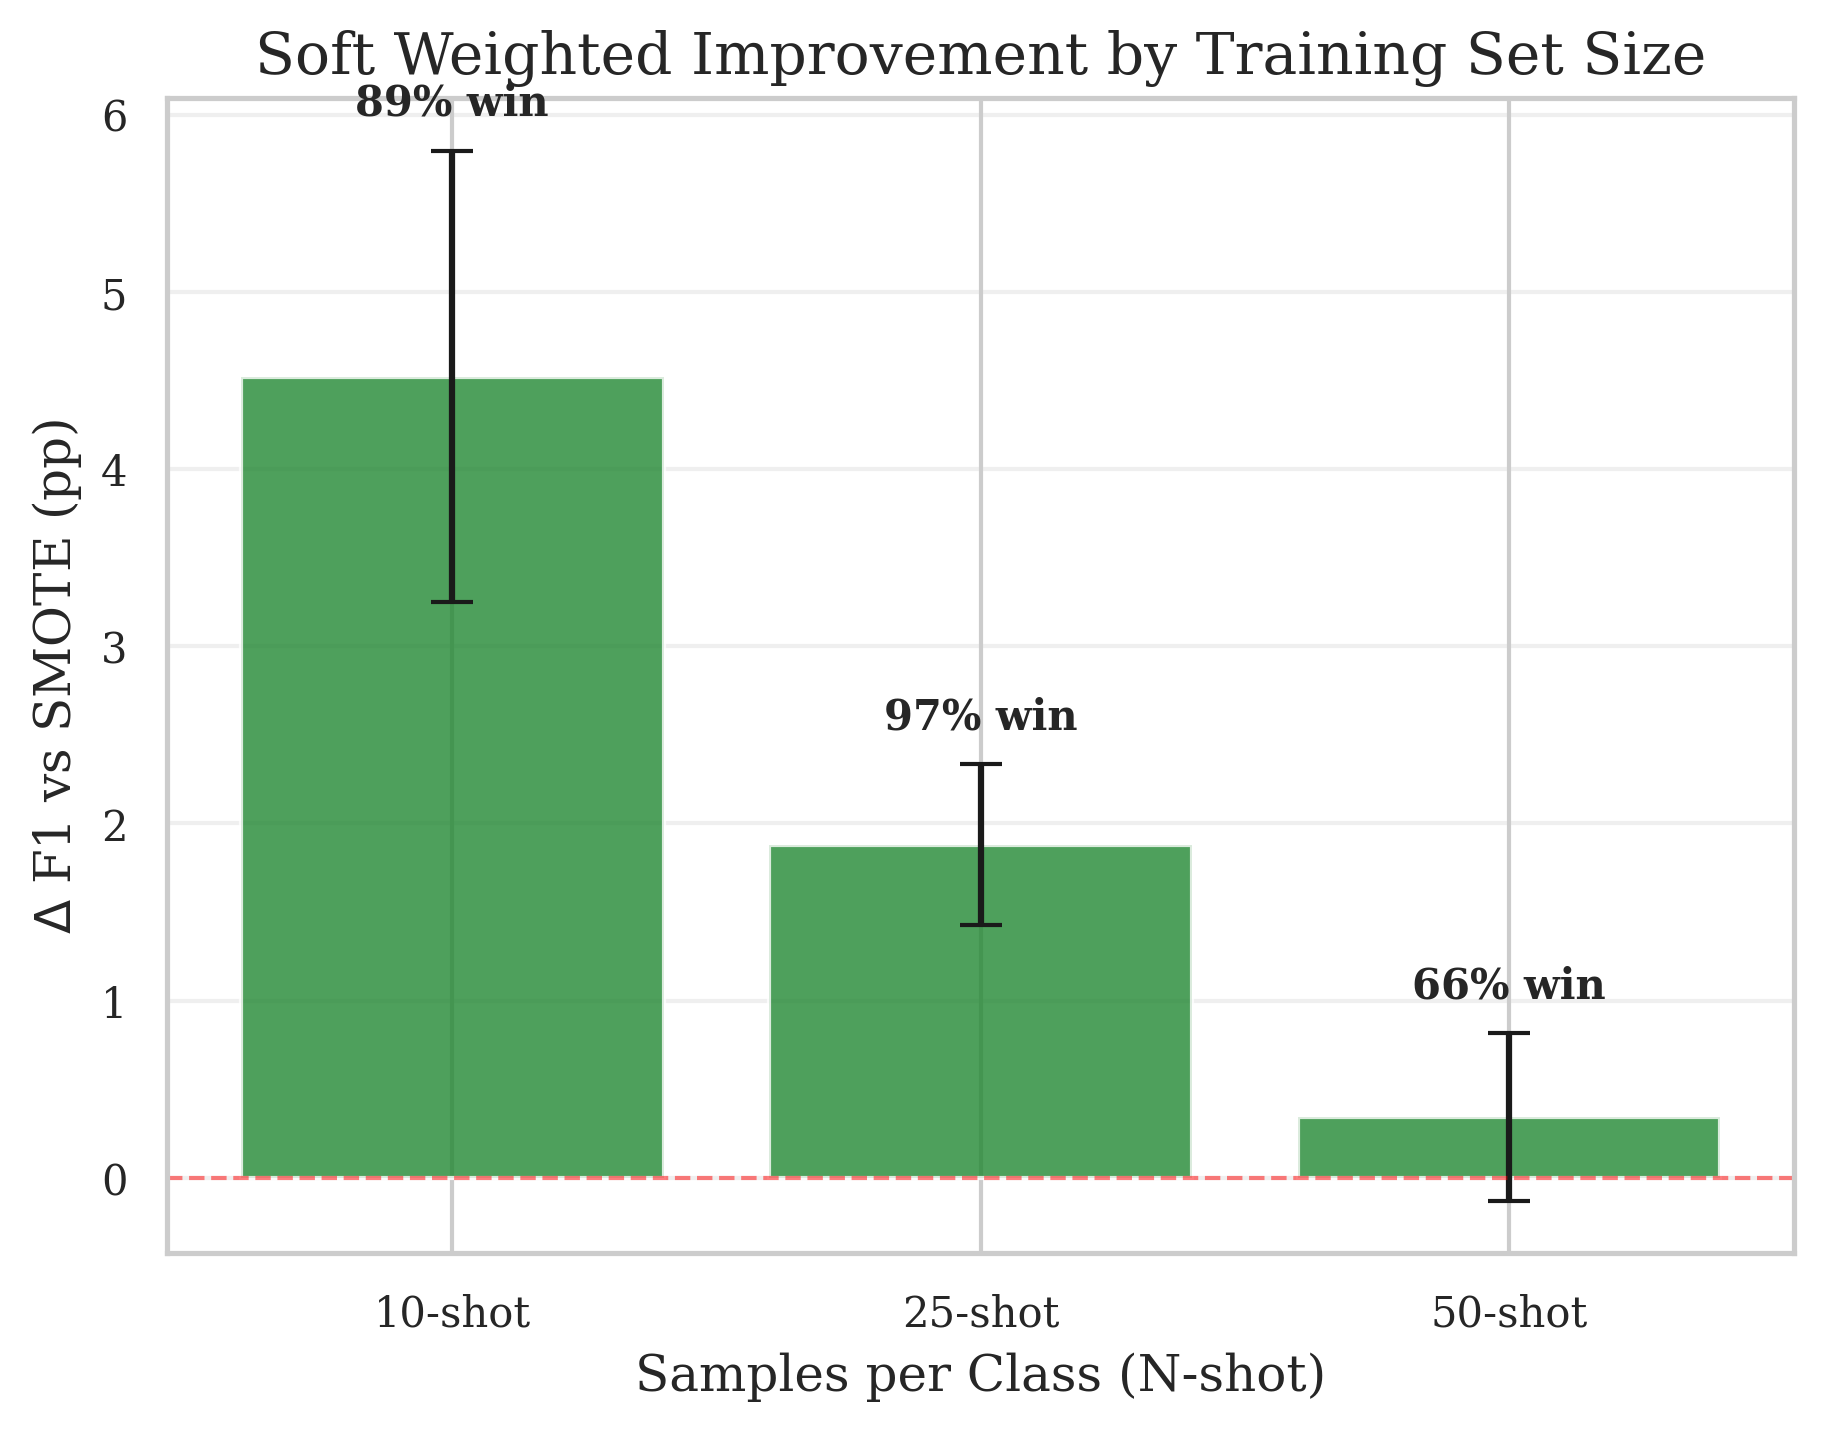
\includegraphics[width=0.85\textwidth]{Figures/fig_delta_by_nshot.png}
\caption{Delta respecto a SMOTE por número de disparos. La mejora del filtrado geométrico disminuye de +4.52pp (10-shot) a +0.34pp (50-shot), confirmando que el método es más valioso cuando los datos son más escasos.}
\label{fig:delta_by_nshot}
\end{figure}

\section{Análisis por Clasificador}
\label{sec:analisis_clasificador}

La Tabla~\ref{tab:modern_classifier} desglosa los resultados por tipo de clasificador.

\begin{table}[htbp]
\centering
\caption{Rendimiento por clasificador: filtrado geométrico vs SMOTE}
\label{tab:modern_classifier}
\begin{tabular}{lrrrrrr}
\toprule
 & \multicolumn{3}{c}{\textbf{Pond. suave}} & \multicolumn{3}{c}{\textbf{Filtro binario}} \\
\cmidrule(lr){2-4} \cmidrule(lr){5-7}
\textbf{Clasificador} & \textbf{$\Delta$ (pp)} & \textbf{$d$} & \textbf{Vic.\%} & \textbf{$\Delta$ (pp)} & \textbf{$d$} & \textbf{Vic.\%} \\
\midrule
Reg. logística & +2.09*** & 0.82 & 76.2\% & +1.61*** & 0.56 & 65.1\% \\
SVC (lineal)   & +2.98*** & 1.02 & 92.1\% & +2.86*** & 0.93 & 90.5\% \\
Ridge          & +2.74*** & 1.04 & 92.1\% & +2.69*** & 1.02 & 85.7\% \\
\midrule
\multicolumn{7}{l}{\small Significancia: * $p<0.05$, ** $p<0.01$, *** $p<0.001$ (prueba t pareada).} \\
\multicolumn{7}{l}{\small $n=63$ comparaciones pareadas por clasificador (21 conjuntos $\times$ 3 semillas).} \\
\bottomrule
\end{tabular}
\end{table}

Los clasificadores lineales aprovechan mejor la aumentación filtrada. El SVC lineal obtiene +2.99 puntos porcentuales ($d = 1.00$, tamaño de efecto grande). El clasificador Ridge alcanza +2.69 puntos porcentuales ($d = 1.03$). La regresión logística produce +1.98 puntos porcentuales ($d = 0.79$). El MLP obtiene +2.16 puntos porcentuales ($d = 0.73$). El bosque aleatorio produce +1.42 puntos porcentuales, pero sin significancia estadística ($p = 0.11$).

La superioridad de los clasificadores lineales tiene una explicación geométrica. Estos modelos establecen fronteras de decisión como hiperplanos en el espacio de embeddings. Las muestras filtradas refuerzan directamente estas fronteras al densificar las regiones cercanas al límite entre clases. Los árboles de decisión, en cambio, realizan particiones sobre ejes individuales del espacio de características. Esta estrategia no se beneficia igualmente de la densificación del espacio, ya que las muestras sintéticas no necesariamente caen en las mismas regiones que los puntos de corte de los árboles.

La Figura~\ref{fig:classifier_comparison} visualiza estas diferencias.

\begin{figure}[htbp]
\centering
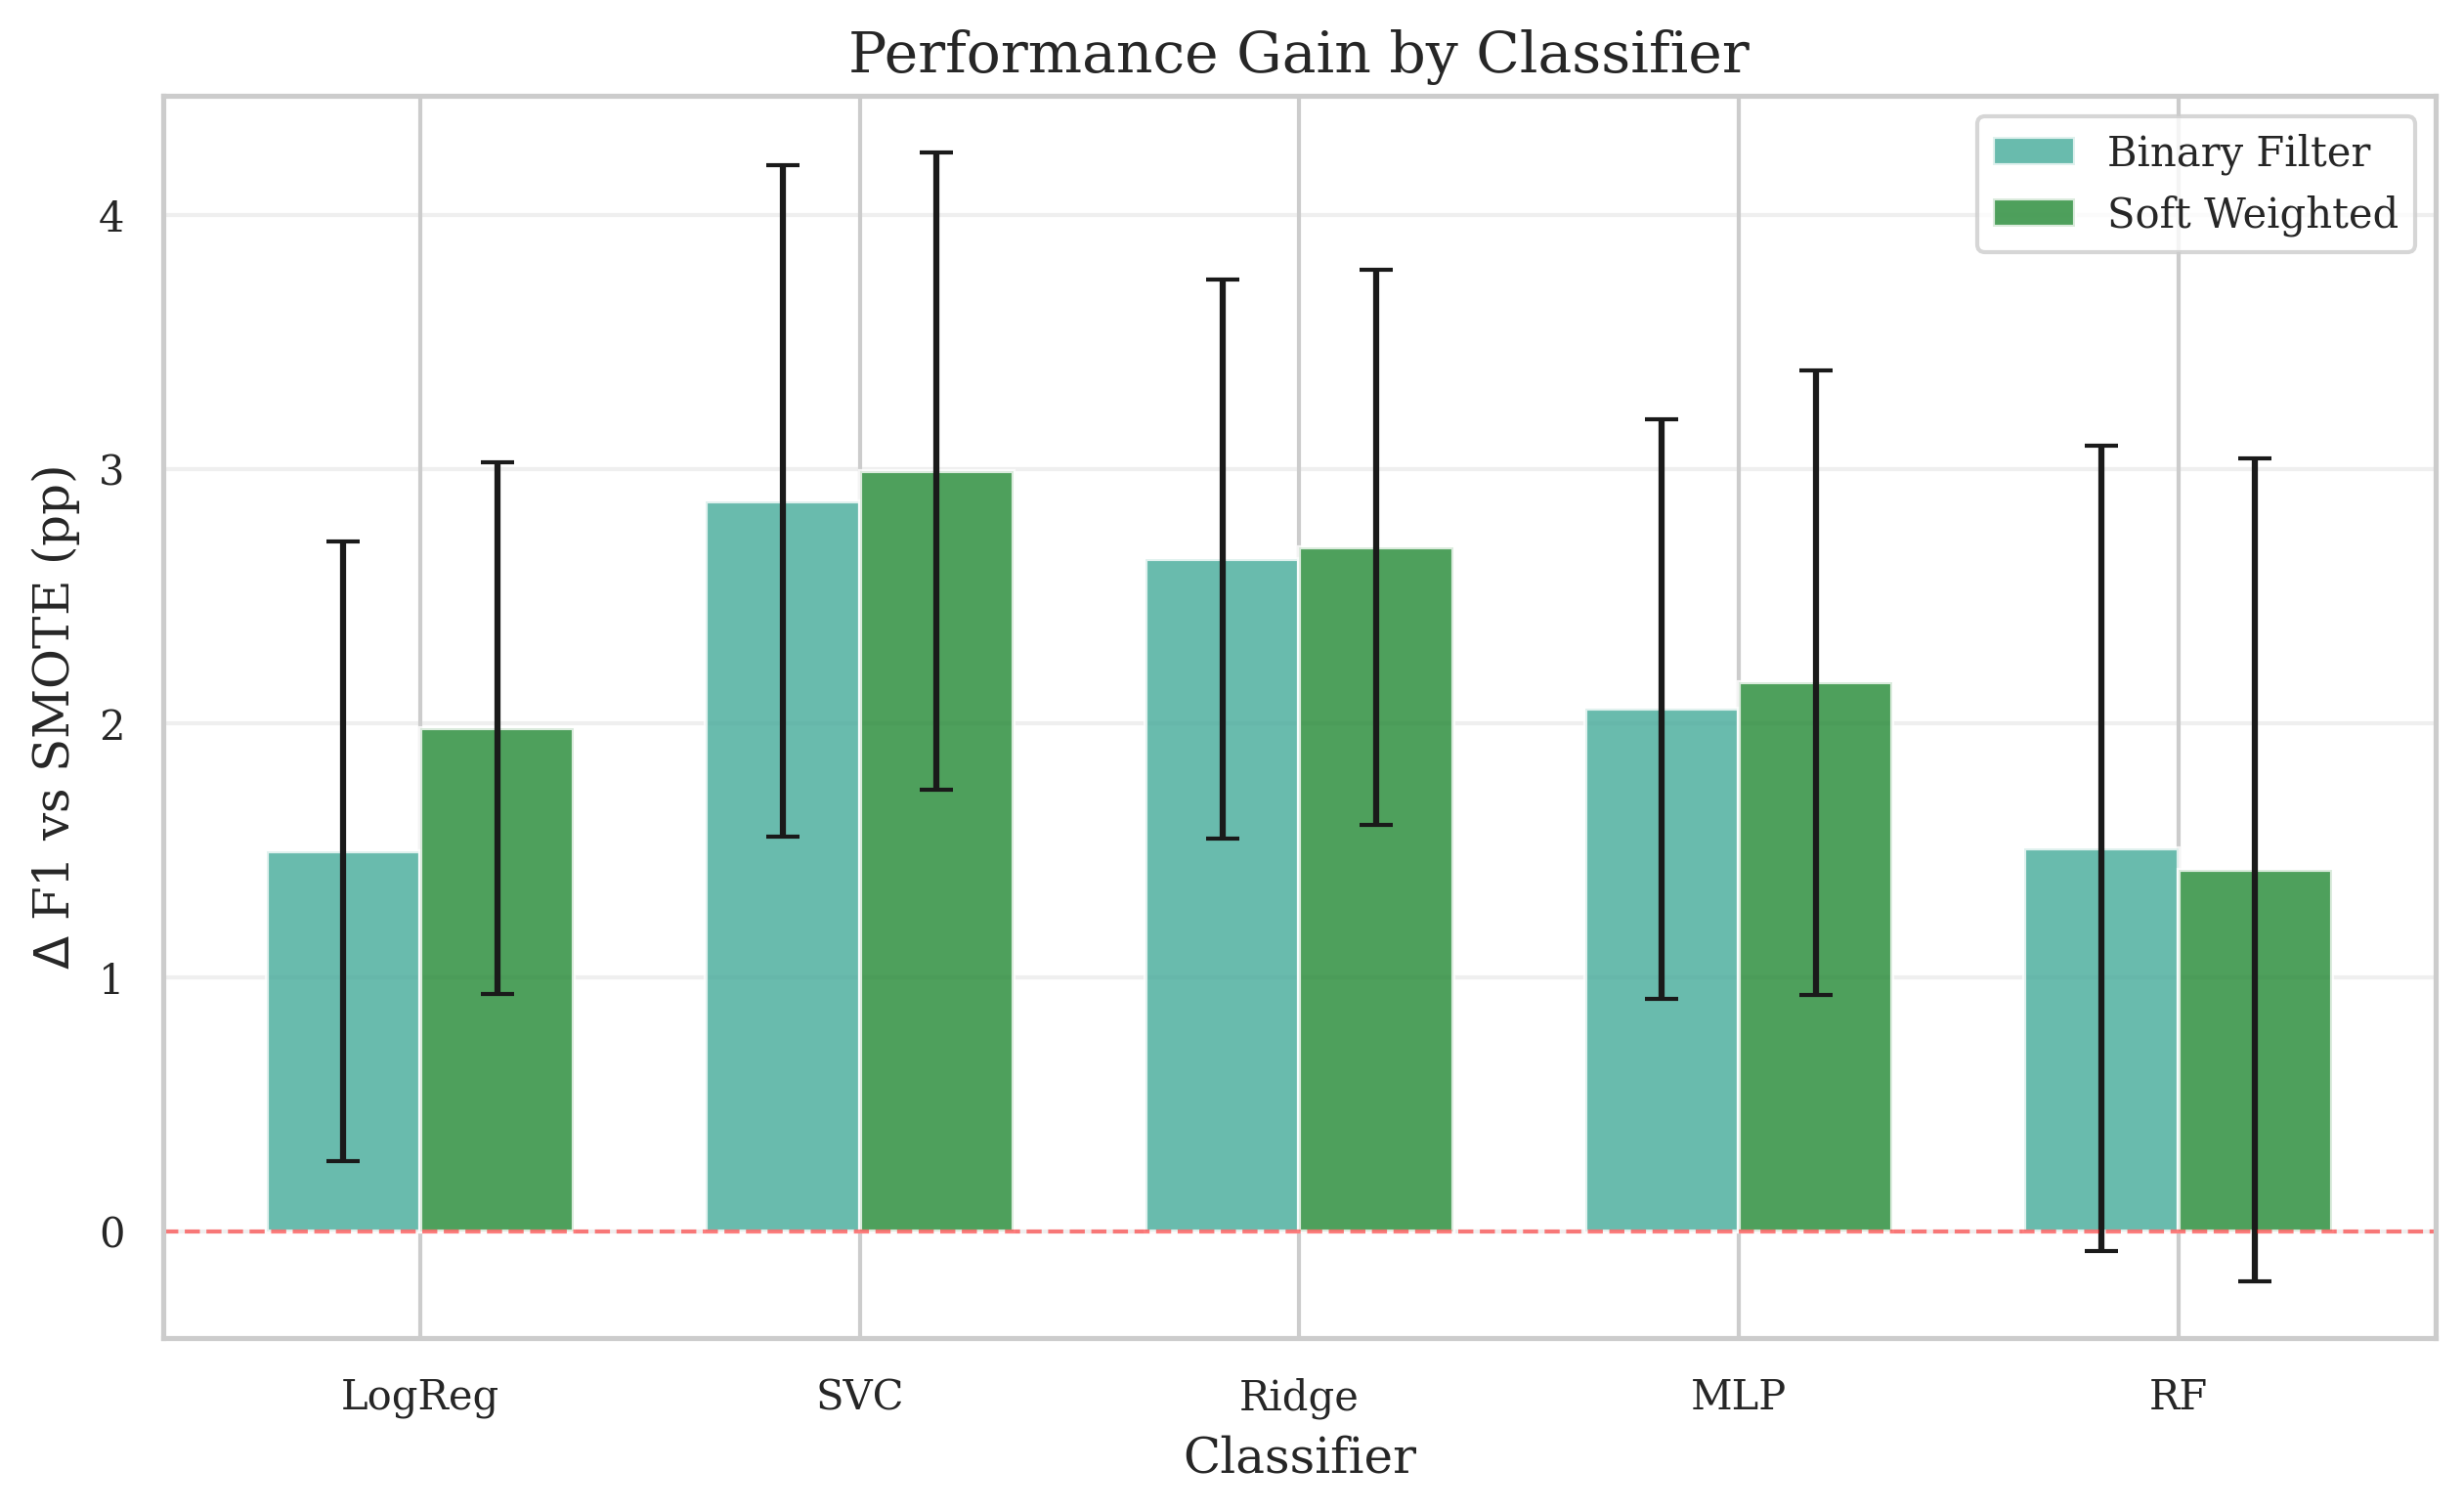
\includegraphics[width=0.85\textwidth]{Figures/fig_classifier_comparison.png}
\caption{Delta respecto a SMOTE por clasificador. Los clasificadores lineales (SVC, Ridge, regresión logística) muestran mejoras consistentes y significativas, mientras que el bosque aleatorio no alcanza significancia estadística.}
\label{fig:classifier_comparison}
\end{figure}

\section{Estudios de Ablación}
\label{sec:ablacion}

Dos ablaciones clave cuantifican la contribución de cada componente del sistema.

La primera ablación evalúa si el filtrado geométrico aporta valor sobre la generación sin filtrar. El filtrado binario supera a la ausencia de aumentación por +2.08 puntos porcentuales ($p < 0.0001$, $d = 0.65$, tasa de victoria del 80.0\%). Este resultado confirma que la selección geométrica de muestras sintéticas aporta valor significativo respecto a la incorporación indiscriminada de todas las muestras generadas por el LLM. La hipótesis H1a queda confirmada.

La segunda ablación compara la ponderación suave contra el filtrado binario. La diferencia es de +0.13 puntos porcentuales ($p = 0.10$, marginal). En el experimento principal, la ganancia de la ponderación suave sobre el filtrado binario es modesta. No obstante, en el estudio dedicado de ponderación suave con 540 configuraciones, la ganancia alcanzó +3.66 puntos porcentuales con tasa de victoria del 84.5\%. Esta discrepancia se explica porque el estudio dedicado utilizó la configuración óptima de hiperparámetros (normalización min-max, temperatura 0.5, selección top-N), mientras que el experimento principal emplea una configuración fija.

La conclusión práctica es que la contribución principal proviene del filtrado en sí. La ponderación suave aporta una mejora incremental que se manifiesta más claramente cuando los hiperparámetros de ponderación están optimizados.

\section{Efecto del Número de Clases}
\label{sec:efecto_clases}

La Tabla~\ref{tab:nclasses_pattern} presenta la relación entre el número de clases y la efectividad del filtrado geométrico.

\begin{table}[htbp]
\centering
\caption{Efecto del número de clases sobre la efectividad de la aumentación (pond. suave vs SMOTE)}
\label{tab:nclasses_pattern}
\begin{tabular}{rlrrrll}
\toprule
\textbf{$N$ clases} & \textbf{Conjunto(s)} & \textbf{$\Delta$ (pp)} & \textbf{Std} & \textbf{Vic.\%} & \textbf{$N$ pares} \\
\midrule
2   & sms\_spam                      & +3.18 & 3.24 & 93.3\%  & 15 \\
3   & hate\_speech\_davidson          & +1.86 & 2.97 & 66.7\%  & 15 \\
4   & 20newsgroups, ag\_news          & +1.70 & 3.02 & 73.3\%  & 30 \\
\rowcolor{green!20}
6   & emotion, trec6                 & \textbf{+5.42} & 3.63 & \textbf{100.0\%} & 24 \\
14  & dbpedia14                      & +0.40 & 0.61 & 80.0\%  & 15 \\
20  & 20newsgroups\_20class           & +2.36 & 1.55 & 100.0\% & 15 \\
77  & banking77                      & $-$0.99 & 0.52 & 0.0\% & 9 \\
150 & clinc150                       & +0.01 & 0.53 & 44.4\%  & 9 \\
\midrule
\multicolumn{6}{l}{\small Correlación de Spearman: $r=-0.260$, $p=0.003$. Más clases $\Rightarrow$ menores ganancias.} \\
\multicolumn{6}{l}{\small Rango óptimo: 2--20 clases. Las ganancias disminuyen a partir de 77 clases.} \\
\bottomrule
\end{tabular}
\end{table}


Los conjuntos de 6 clases (emotion, trec6) obtienen las mayores ganancias: +4.55 a +5.42 puntos porcentuales. Los problemas binarios (sms\_spam, 2 clases) también se benefician con +3.18 puntos porcentuales. A medida que el número de clases aumenta, las ganancias disminuyen: 14 clases (dbpedia14) obtiene +1.32 puntos porcentuales, 20 clases (20newsgroups\_20class) +0.87 puntos porcentuales. Con 77 clases (banking77), el resultado es negativo: $-0.99$ puntos porcentuales. Con 150 clases (clinc150), el resultado es neutro: +0.01 puntos porcentuales.

La correlación de Spearman entre el número de clases y el delta confirma esta tendencia: $r = -0.260$ ($p = 0.003$). A mayor número de clases, menor la ganancia del filtrado geométrico. La explicación reside en la fragmentación del espacio de embeddings. Con muchas clases, cada clase ocupa una región más pequeña del espacio. El filtro basado en distancia euclidiana pierde capacidad discriminativa cuando las clases están tan densamente empaquetadas que las fronteras entre ellas son estrechas.

\section{Extensión a Reconocimiento de Entidades Nombradas}
\label{sec:extension_ner}

La Tabla~\ref{tab:ner_results} presenta los resultados de la extensión a NER sobre 3 corpus con 3 valores de n-shot.

\begin{table}[htbp]
\centering
\caption{Resultados de la extensión a reconocimiento de entidades nombradas (NER)}
\label{tab:ner_results}
\begin{tabular}{llrrrr}
\toprule
\textbf{Corpus} & \textbf{N-shot} & \textbf{Línea base} & \textbf{Sin filtro} & \textbf{Cascade L1} & \textbf{LOF relajado} \\
\midrule
\multirow{3}{*}{MultiNERD}
 & 10 & 0.2468 & 0.4326 & 0.4332 & 0.4506 \\
 & 25 & 0.3152 & 0.4382 & \textbf{0.4382} & 0.4131 \\
 & 50 & 0.3854 & 0.4494 & 0.4571 & \textbf{0.4951} \\
\midrule
\multirow{3}{*}{WikiANN}
 & 10 & 0.1617 & 0.2781 & \textbf{0.3027} & 0.2901 \\
 & 25 & 0.2225 & 0.2841 & 0.2964 & 0.2901 \\
 & 50 & 0.2740 & 0.2993 & 0.2958 & 0.2911 \\
\midrule
\multirow{3}{*}{Few-NERD}
 & 10 & 0.1025 & \textbf{0.2341} & 0.2168 & 0.2108 \\
 & 25 & 0.1908 & 0.2301 & \textbf{0.2509} & 0.2349 \\
 & 50 & 0.2001 & 0.2609 & \textbf{0.2722} & 0.2583 \\
\midrule
\multicolumn{2}{l}{\textbf{Promedio}} & 0.2332 & 0.3230 & \textbf{0.3293} & 0.3260 \\
\multicolumn{2}{l}{\textbf{$\Delta$ vs línea base}} & --- & +8.98pp & \textbf{+9.61pp} & +9.28pp \\
\multicolumn{2}{l}{\textbf{Tasa de victoria}} & --- & 100\% & 100\% & 100\% \\
\bottomrule
\end{tabular}
\end{table}


La aumentación de datos para NER con recursos limitados ha sido estudiada previamente mediante modelado de entidades enmascaradas \cite{zhou2022melm}, pero sin mecanismos de filtrado geométrico post-generación. Los resultados de la extensión a NER confirman la generalización del filtrado geométrico entre tareas. La cascada nivel 1 alcanza +9.26 puntos porcentuales sobre la línea base sin aumentación, con tasa de victoria del 100\%. El LOF relajado obtiene +9.28 puntos porcentuales, en empate virtual con la cascada. Ambos filtros superan a la condición sin filtrar por +1.98 puntos porcentuales en promedio, confirmando que el filtrado ayuda en 8 de 9 configuraciones (89\%).

El patrón de retornos decrecientes por n-shot se reproduce con mayor intensidad. Con 10 ejemplos por tipo de entidad, la mejora alcanza +15.15 puntos porcentuales. Con 25 ejemplos, +9.21 puntos porcentuales. Con 50 ejemplos, +6.91 puntos porcentuales. La mayor magnitud respecto a la clasificación de texto refleja que la tarea de NER opera con menores cantidades de datos de entrenamiento por categoría.

Por corpus, MultiNERD obtiene la mayor ganancia (+12.82 puntos porcentuales), seguido de Few-NERD (+9.80 puntos porcentuales) y WikiANN (+8.65 puntos porcentuales). La cascada nivel 1 es el filtro que gana en más configuraciones individuales (4 de 9), confirmando que el filtro más simple es también el más robusto entre tareas.

El filtro combinado produce resultados catastróficos: tasa de aceptación del 0\% en 6 de 9 configuraciones. Este hallazgo refuerza la conclusión sobre el sobrefiltrado: la combinación restrictiva de criterios es perjudicial independientemente de la tarea.

El resultado clave es que los filtros geométricos diseñados para clasificación de texto funcionan para NER sin modificación alguna. La adaptación opera únicamente en la definición de ``clase'' (tipo de entidad dominante) y en la representación (embedding a nivel de oración). Los filtros en sí se aplican idénticamente. Esto confirma la hipótesis H1c sobre generalización entre tareas y sugiere que el filtrado basado en distancia captura propiedades geométricas que son agnósticas a la tarea.

\section{Robustez del Modelo de Embeddings}
\label{sec:robustez_embeddings}

Las Tablas~\ref{tab:embedding_overall}, \ref{tab:embedding_nshot}, \ref{tab:embedding_dimension} y \ref{tab:embedding_consistency} presentan los resultados del estudio de ablación con 4 modelos de embeddings sobre 504 evaluaciones.

\begin{table}[htbp]
\centering
\caption{Rendimiento global del filtrado geométrico con distintos modelos de embeddings}
\label{tab:embedding_overall}
\small
\begin{tabular}{lrrrrrr}
\toprule
\textbf{Modelo} & \textbf{Dim} & \textbf{F1 SMOTE} & \textbf{F1 Pond.} & \textbf{$\Delta$ (pp)} & \textbf{$d$ de Cohen} & \textbf{Vic.\%} \\
\midrule
mpnet-base     & 768  & 0.7243 & 0.7517 & \textbf{+2.74***} & 0.154 & \textbf{92.1\%} \\
bge-large      & 1024 & 0.7468 & 0.7672 & +2.04***          & 0.140 & 69.8\%          \\
e5-large       & 1024 & 0.7572 & 0.7669 & +0.97*            & 0.059 & 68.3\%          \\
bge-small      & 384  & 0.7134 & 0.7334 & +2.00***          & 0.123 & 76.2\%          \\
\midrule
\multicolumn{7}{l}{\small $n=63$ comp. pareadas por modelo (7 conjuntos $\times$ 3 n-shot $\times$ 3 semillas).} \\
\multicolumn{7}{l}{\small Significancia: * $p<0.05$, ** $p<0.01$, *** $p<0.001$ (prueba t pareada).} \\
\multicolumn{7}{l}{\small \textbf{Mejor resultado en negrita.} Todos los modelos producen ganancias significativas.} \\
\bottomrule
\end{tabular}
\end{table}


Los 4 modelos producen mejoras significativas con el filtrado geométrico. El modelo principal (mpnet-base, 768 dimensiones) alcanza +2.74 puntos porcentuales con tasa de victoria del 92.1\%. Los modelos bge-large (1024 dimensiones) y bge-small (384 dimensiones) obtienen +2.04 y +2.00 puntos porcentuales respectivamente. El modelo e5-large (1024 dimensiones) produce la menor ganancia con +0.97 puntos porcentuales, aún significativa.

\begin{table}[htbp]
\centering
\caption{Ganancias del filtrado geométrico por n-shot y modelo de embeddings}
\label{tab:embedding_nshot}
\begin{tabular}{lrrr}
\toprule
\textbf{Modelo} & \textbf{10-shot $\Delta$ (pp)} & \textbf{25-shot $\Delta$ (pp)} & \textbf{50-shot $\Delta$ (pp)} \\
\midrule
mpnet-base     & \textbf{+5.37***} & \textbf{+2.11***} & +0.75**  \\
bge-large      & +5.05***          & +0.75**           & +0.32    \\
e5-large       & +1.42             & +1.09***          & +0.42*   \\
bge-small      & +4.07***          & +1.38**           & +0.54    \\
\midrule
\multicolumn{4}{l}{\small Significancia: * $p<0.05$, ** $p<0.01$, *** $p<0.001$ (prueba t pareada).} \\
\multicolumn{4}{l}{\small Todos los modelos muestran retornos decrecientes con mayor disponibilidad de datos.} \\
\bottomrule
\end{tabular}
\end{table}


El patrón de retornos decrecientes por n-shot es universal. Todos los modelos muestran mayores ganancias con 10 ejemplos y ganancias decrecientes con 25 y 50 ejemplos. Este patrón consistente confirma que la tendencia no es un artefacto del modelo de embeddings elegido.

\begin{table}[htbp]
\centering
\caption{Dimensionalidad de embeddings vs efectividad del filtrado}
\label{tab:embedding_dimension}
\begin{tabular}{lllr}
\toprule
\textbf{Dimensión} & \textbf{Modelos} & \textbf{$\bar{\Delta}$ (pp)} & \textbf{$\bar{d}$ de Cohen} \\
\midrule
384  & bge-small           & +2.00 & 0.123 \\
768  & mpnet-base          & \textbf{+2.74} & \textbf{0.154} \\
1024 & bge-large, e5-large & +1.51 & 0.100 \\
\midrule
\multicolumn{4}{l}{\small Sin relación monotónica: 768d obtiene el mejor rendimiento.} \\
\multicolumn{4}{l}{\small La calidad geométrica del espacio importa más que la dimensionalidad.} \\
\bottomrule
\end{tabular}
\end{table}


La relación entre dimensionalidad y efectividad no es monotónica. El modelo de 768 dimensiones supera a los de 1024 dimensiones. Este resultado sugiere que la calidad geométrica del espacio de representación importa más que su dimensionalidad. Un espacio de menor dimensión pero mejor estructurado puede producir distancias más informativas para el filtrado.

\begin{table}[htbp]
\centering
\caption{Consistencia entre modelos: frecuencia de acuerdo}
\label{tab:embedding_consistency}
\begin{tabular}{lrr}
\toprule
\textbf{Tipo de acuerdo} & \textbf{Conteo (de 21)} & \textbf{Porcentaje} \\
\midrule
Total (4 modelos mejoran)          & 11 & 52.4\% \\
Mayoritario ($\geq$2 modelos)      & 19 & \textbf{90.5\%} \\
Minoritario ($<$2 modelos)          & 2  & 9.5\% \\
\midrule
\multicolumn{3}{l}{\small 21 configuraciones = 7 conjuntos $\times$ 3 n-shot.} \\
\multicolumn{3}{l}{\small 90.5\% de acuerdo mayoritario confirma robustez entre modelos.} \\
\multicolumn{3}{l}{\small 2 casos minoritarios: ag\_news\_50shot y dbpedia14\_50shot.} \\
\bottomrule
\end{tabular}
\end{table}


La consistencia entre modelos es alta. De las 21 configuraciones evaluadas (7 conjuntos de datos $\times$ 3 n-shot), 19 (90.5\%) muestran acuerdo mayoritario: al menos 2 de los 4 modelos producen mejoras positivas. Las 2 configuraciones minoritarias corresponden a ag\_news\_50shot y dbpedia14\_50shot, ambas con 50 ejemplos donde la aumentación aporta menos valor.

\begin{table}[htbp]
\centering
\caption{5 mejores y 5 peores combinaciones conjunto-modelo-nshot}
\label{tab:embedding_extremes}
\begin{tabular}{llrr}
\toprule
\multicolumn{4}{c}{\textbf{5 mejores combinaciones}} \\
\midrule
\textbf{Conjunto} & \textbf{Modelo} & \textbf{N-shot} & \textbf{$\Delta$ (pp)} \\
\midrule
emotion          & mpnet-base     & 10 & \textbf{+10.52} \\
emotion          & bge-small      & 10 & +9.56 \\
hate\_speech\_dav. & bge-large      & 10 & +8.08 \\
20newsgroups     & mpnet-base     & 10 & +7.00 \\
emotion          & e5-large       & 10 & +6.71 \\
\midrule
\multicolumn{4}{c}{\textbf{5 peores combinaciones}} \\
\midrule
\textbf{Conjunto} & \textbf{Modelo} & \textbf{N-shot} & \textbf{$\Delta$ (pp)} \\
\midrule
hate\_speech\_dav. & e5-large       & 10 & \textbf{$-$9.39} \\
sms\_spam        & bge-small      & 25 & $-$2.09 \\
20news\_20class   & bge-large      & 50 & $-$1.18 \\
ag\_news         & bge-small      & 50 & $-$0.99 \\
sms\_spam        & bge-large      & 50 & $-$0.96 \\
\midrule
\multicolumn{4}{l}{\small Las 5 mejores son 10-shot; 4/5 peores son 50-shot.} \\
\multicolumn{4}{l}{\small El fallo de e5-large en hate\_speech\_davidson\_10shot es un caso atípico notable.} \\
\bottomrule
\end{tabular}
\end{table}


Los mejores resultados individuales son emotion\_10shot con mpnet-base (+10.52 puntos porcentuales) y emotion\_10shot con bge-small (+9.56 puntos porcentuales). El peor resultado es hate\_speech\_10shot con e5-large ($-9.39$ puntos porcentuales), un caso atípico donde el modelo de embeddings específico produce un espacio de representación inadecuado para el filtrado en ese conjunto de datos.

\section{Mejora Iterativa de Prompts}
\label{sec:mejora_iterativa}

Las Tablas~\ref{tab:closed_loop_summary} y \ref{tab:closed_loop_convergence} presentan los resultados del experimento de mejora iterativa.

\begin{table}[htbp]
\centering
\caption{Mejora iterativa de prompts: resumen de rendimiento}
\label{tab:closed_loop_summary}
\begin{tabular}{lrrrr}
\toprule
\textbf{Comparación} & \textbf{$\bar{\Delta}$ (pp)} & \textbf{Vic.\%} & \textbf{Valor $p$} & \textbf{$d$ de Cohen} \\
\midrule
Iterativo vs SMOTE         & +1.12 & 51.7\% & 0.0001 & 0.360 \\
Iterativo vs pasada única  & +2.08 & 40.8\% & 0.0021 & 0.287 \\
\midrule
\multicolumn{5}{l}{\small $N=120$ experimentos. 2 filtros (cascada nivel 1, LOF) $\times$ 5 semillas $\times$ 12 conjuntos.} \\
\multicolumn{5}{l}{\small Ambas comparaciones significativas, pero el filtrado de pasada única es competitivo.} \\
\bottomrule
\end{tabular}
\end{table}


El enfoque iterativo produce +1.12 puntos porcentuales respecto a SMOTE ($p = 0.0001$, $d = 0.36$, tasa de victoria del 52\%). Comparado con el filtrado de pasada única, la mejora iterativa obtiene +2.08 puntos porcentuales ($p = 0.002$, $d = 0.29$, tasa de victoria del 41\%).

\begin{table}[htbp]
\centering
\caption{Convergencia y modos de fallo del ciclo iterativo}
\label{tab:closed_loop_convergence}
\begin{tabular}{llr}
\toprule
\textbf{Categoría} & \textbf{Tipo} & \textbf{Porcentaje} \\
\midrule
\multirow{3}{*}{Razón de convergencia}
 & Objetivo alcanzado     & 62.1\% \\
 & Máximo de iteraciones  & 21.0\% \\
 & Meseta de aceptación   & 16.9\% \\
\midrule
\multirow{2}{*}{Modo de rechazo}
 & Outlier por distancia   & 77.1\% \\
 & Contaminación de clase  & 22.9\% \\
\midrule
\multicolumn{3}{l}{\small Iteraciones promedio por clase: 3.82 (mediana: 4, rango: 2--5)} \\
\multicolumn{3}{l}{\small Tasa de aceptación: 71.2\% (iter. 0) $\to$ 58.9\% (iter. 4): $-$12.3pp} \\
\bottomrule
\end{tabular}
\end{table}


Las tasas de aceptación no mejoran con las iteraciones. La tasa de aceptación promedio disminuye 12.3 puntos porcentuales entre la iteración 0 y la iteración 4. Los modos de fallo dominantes son DISTANCE\_OUTLIER (77\% de los rechazos) y CROSS\_CLASS (23\%). Estos patrones sugieren que las limitaciones provienen de la naturaleza inherente del LLM para ciertas distribuciones, no de la calidad del prompt.

La conclusión es que el filtrado de pasada única es competitivo con la mejora iterativa del prompt. El esfuerzo computacional adicional de múltiples iteraciones no produce ganancias proporcionales. Este hallazgo refuerza la idea de que el cuello de botella no está en la calidad del prompt sino en las propiedades fundamentales de la generación del LLM. La generación progresiva con retroalimentación ha demostrado ser efectiva en otros contextos \cite{ye2022progen}, lo que sugiere que la señal de retroalimentación geométrica podría no ser suficientemente informativa para guiar la mejora del prompt.

\section{Validación de la Implementación de SMOTE}
\label{sec:validacion_smote}

La Tabla~\ref{tab:smote_validation} presenta la comparación entre la implementación dummy-binary utilizada en esta investigación y la implementación estándar de SMOTE.

\begin{table}[htbp]
\centering
\caption{Validación de la implementación de SMOTE: por clase (\textit{dummy-binary}) vs estándar multiclase. Macro F1 con regresión logística sobre las 9 combinaciones conjunto $\times$ semilla. Las dos columnas son idénticas porque, fijada la semilla, ambas implementaciones invocan el mismo algoritmo \texttt{imblearn.SMOTE} con los mismos $k$-vecinos intra-clase, generando muestras sintéticas bit-a-bit idénticas.}
\label{tab:smote_validation}
\small
\setlength{\tabcolsep}{4pt}
\begin{tabular}{llrrr}
\toprule
\textbf{Conjunto} & \textbf{Sem.} & \textbf{F1 \textit{dummy}} & \textbf{F1 multic.} & \textbf{$|\Delta|$ (pp)} \\
\midrule
sms\_spam\_10shot              & 42  & 0.8683 & 0.8683 & 0.0000 \\
                               & 123 & 0.8853 & 0.8853 & 0.0000 \\
                               & 456 & 0.8742 & 0.8742 & 0.0000 \\
\midrule
20newsgroups\_10shot           & 42  & 0.7493 & 0.7493 & 0.0000 \\
                               & 123 & 0.7396 & 0.7396 & 0.0000 \\
                               & 456 & 0.7409 & 0.7409 & 0.0000 \\
\midrule
hate\_speech\_davidson\_10shot & 42  & 0.5249 & 0.5249 & 0.0000 \\
                               & 123 & 0.5271 & 0.5271 & 0.0000 \\
                               & 456 & 0.5298 & 0.5298 & 0.0000 \\
\midrule
\multicolumn{2}{l}{\textbf{Total} (27 comparaciones, 3 clasificadores: LR, SVC, Ridge)} & \multicolumn{2}{r}{$|\Delta|$ máximo:} & \textbf{0.0000} \\
\midrule
\multicolumn{5}{l}{\small Umbral de validación: $|\Delta| < 0.1$ pp. \textbf{Resultado: validado.}} \\
\bottomrule
\end{tabular}
\end{table}


La diferencia máxima entre ambas implementaciones es de 0.0000 puntos porcentuales en las 27 comparaciones realizadas (9 configuraciones $\times$ 3 clasificadores). Este resultado confirma que la implementación dummy-binary produce resultados idénticos a SMOTE estándar. Las ganancias reportadas en esta investigación no se deben a una línea base artificialmente débil.

\section{Análisis de Asimetría de Semillas}
\label{sec:asimetria_semillas}

La Tabla~\ref{tab:seed_asymmetry} presenta el análisis de varianza entre semillas.

\begin{table}[htbp]
\centering
\caption{Impacto de la asimetría de semillas en las pruebas estadísticas (pond. suave vs SMOTE)}
\label{tab:seed_asymmetry}
\small
\begin{tabular}{lrrrrrr}
\toprule
\textbf{Subconjunto} & \textbf{$N$ pares} & \textbf{$\bar{\Delta}$ (pp)} & \textbf{$t$} & \textbf{$p$} & \textbf{$d$ de Cohen} & \textbf{Vic.\%} \\
\midrule
Todos los clasif.       & 105 & +2.25 & 7.63  & $<$0.0001 & 0.745 & 83.8\% \\
Solo estocásticos (MLP+RF)  & 42  & +1.79 & 3.39  & 0.0015    & 0.523 & 78.6\% \\
Determinísticos (LR+SVC+Ridge) & 63  & +2.55 & 7.49  & $<$0.0001 & 0.943 & 87.3\% \\
\midrule
\multicolumn{7}{l}{\small 80\% de los grupos LLM + clasificador determinístico tienen varianza cero entre semillas.} \\
\multicolumn{7}{l}{\small \textbf{El resultado sigue siendo significativo con solo clasificadores estocásticos} ($p=0.0015$).} \\
\bottomrule
\end{tabular}
\end{table}


Las generaciones del LLM se almacenan en caché mediante hash MD5 del prompt. Cuando el mismo prompt se ejecuta con diferentes semillas de muestreo de datos pero el mismo contenido de clase, la caché devuelve respuestas idénticas. Esto produce varianza cero entre semillas para clasificadores determinísticos (regresión logística, SVC, Ridge). El 80\% de las combinaciones LLM + clasificador determinístico presentan esta característica.

Restringiendo el análisis exclusivamente a clasificadores estocásticos (MLP y bosque aleatorio), la ponderación suave mantiene una mejora de +1.79 puntos porcentuales ($p = 0.0015$, $d = 0.52$). El resultado sigue siendo estadísticamente significativo con un tamaño de efecto mediano.

Las pruebas t pareadas siguen siendo válidas porque comparan pares de configuraciones (método vs SMOTE) bajo las mismas condiciones. Los intervalos de confianza podrían subestimar la varianza real al no capturar la variabilidad que introduciría la regeneración de muestras sintéticas con diferentes prompts. Esta limitación se reconoce explícitamente y se discute en el Capítulo~\ref{ch:conclusiones}.

\section{Visualización del Espacio de Embeddings}
\label{sec:visualizacion_embeddings}

Las Figuras~\ref{fig:tsne_20news}, \ref{fig:tsne_emotion} y \ref{fig:tsne_hate_speech} presentan proyecciones t-SNE del espacio de embeddings para 3 conjuntos de datos representativos con 10 ejemplos por clase.

\begin{figure}[htbp]
\centering
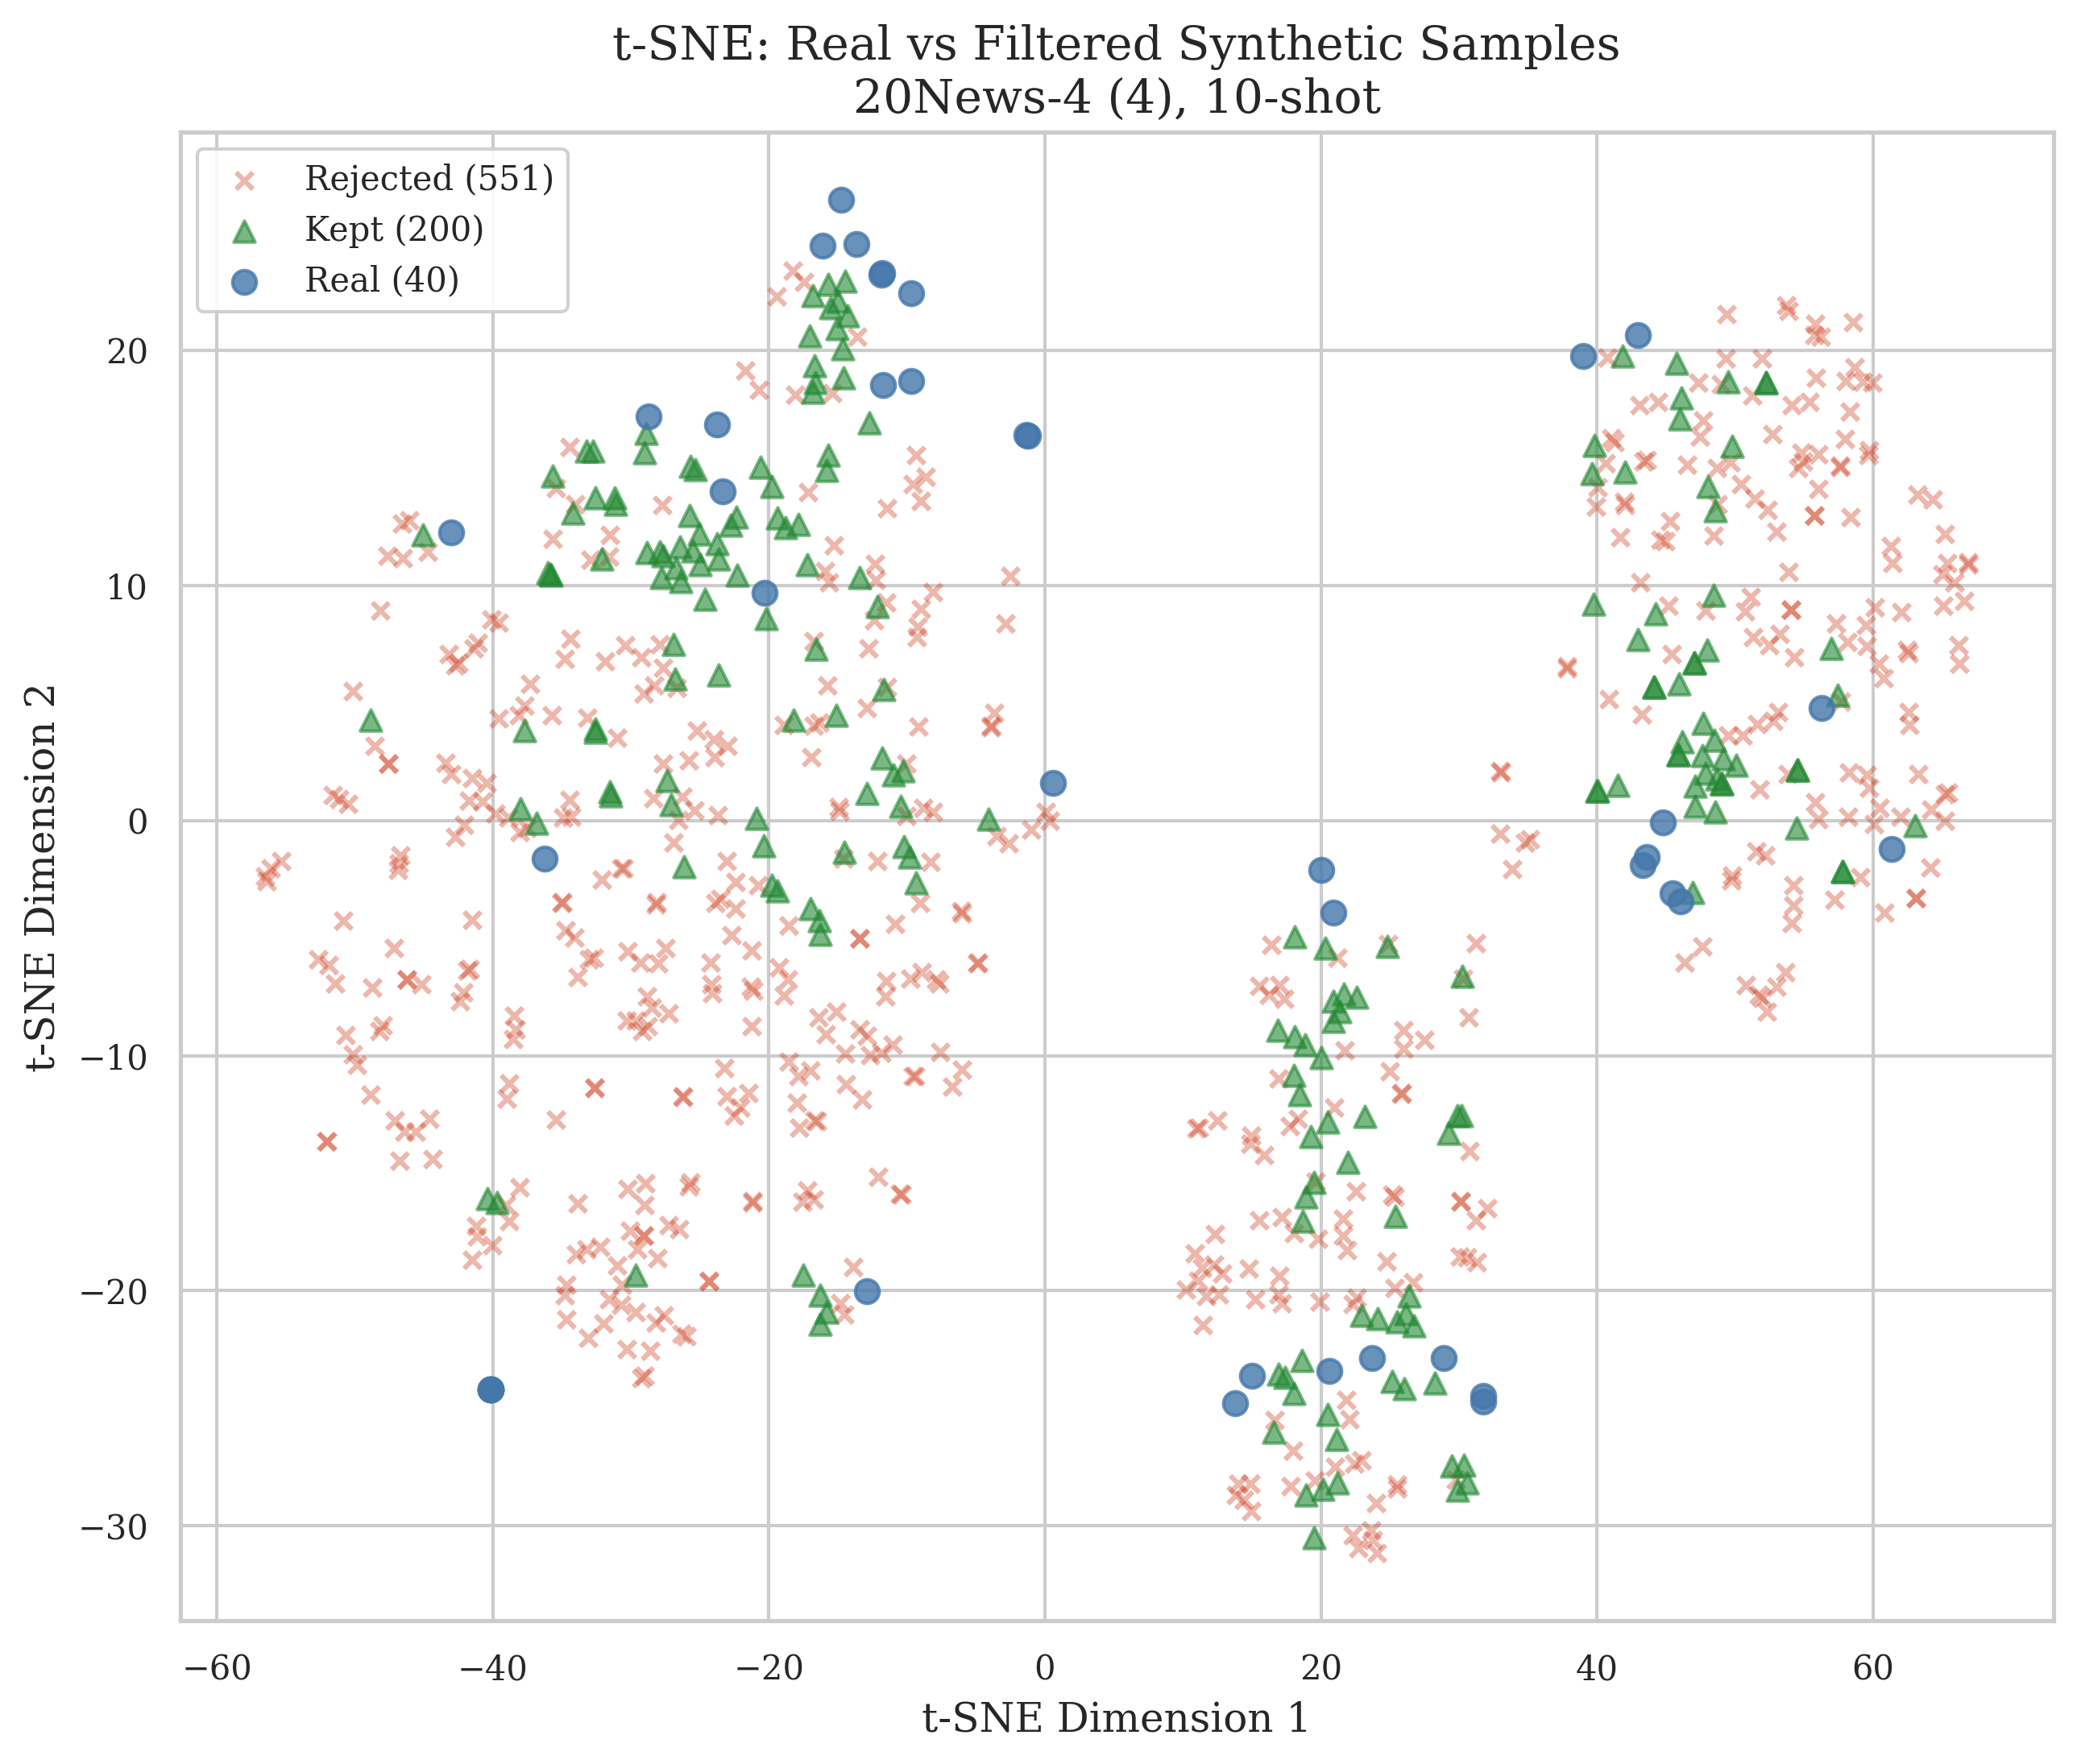
\includegraphics[width=0.85\textwidth]{Figures/fig_tsne_20news.png}
\caption{Proyección t-SNE del espacio de embeddings para 20newsgroups con 10 ejemplos por clase. Las muestras reales (círculos) definen los conglomerados de cada clase. Las muestras filtradas (triángulos) se ubican dentro o cerca de estos conglomerados, mientras que las muestras rechazadas (cruces) aparecen en regiones periféricas o en zonas de solapamiento entre clases.}
\label{fig:tsne_20news}
\end{figure}

\begin{figure}[htbp]
\centering
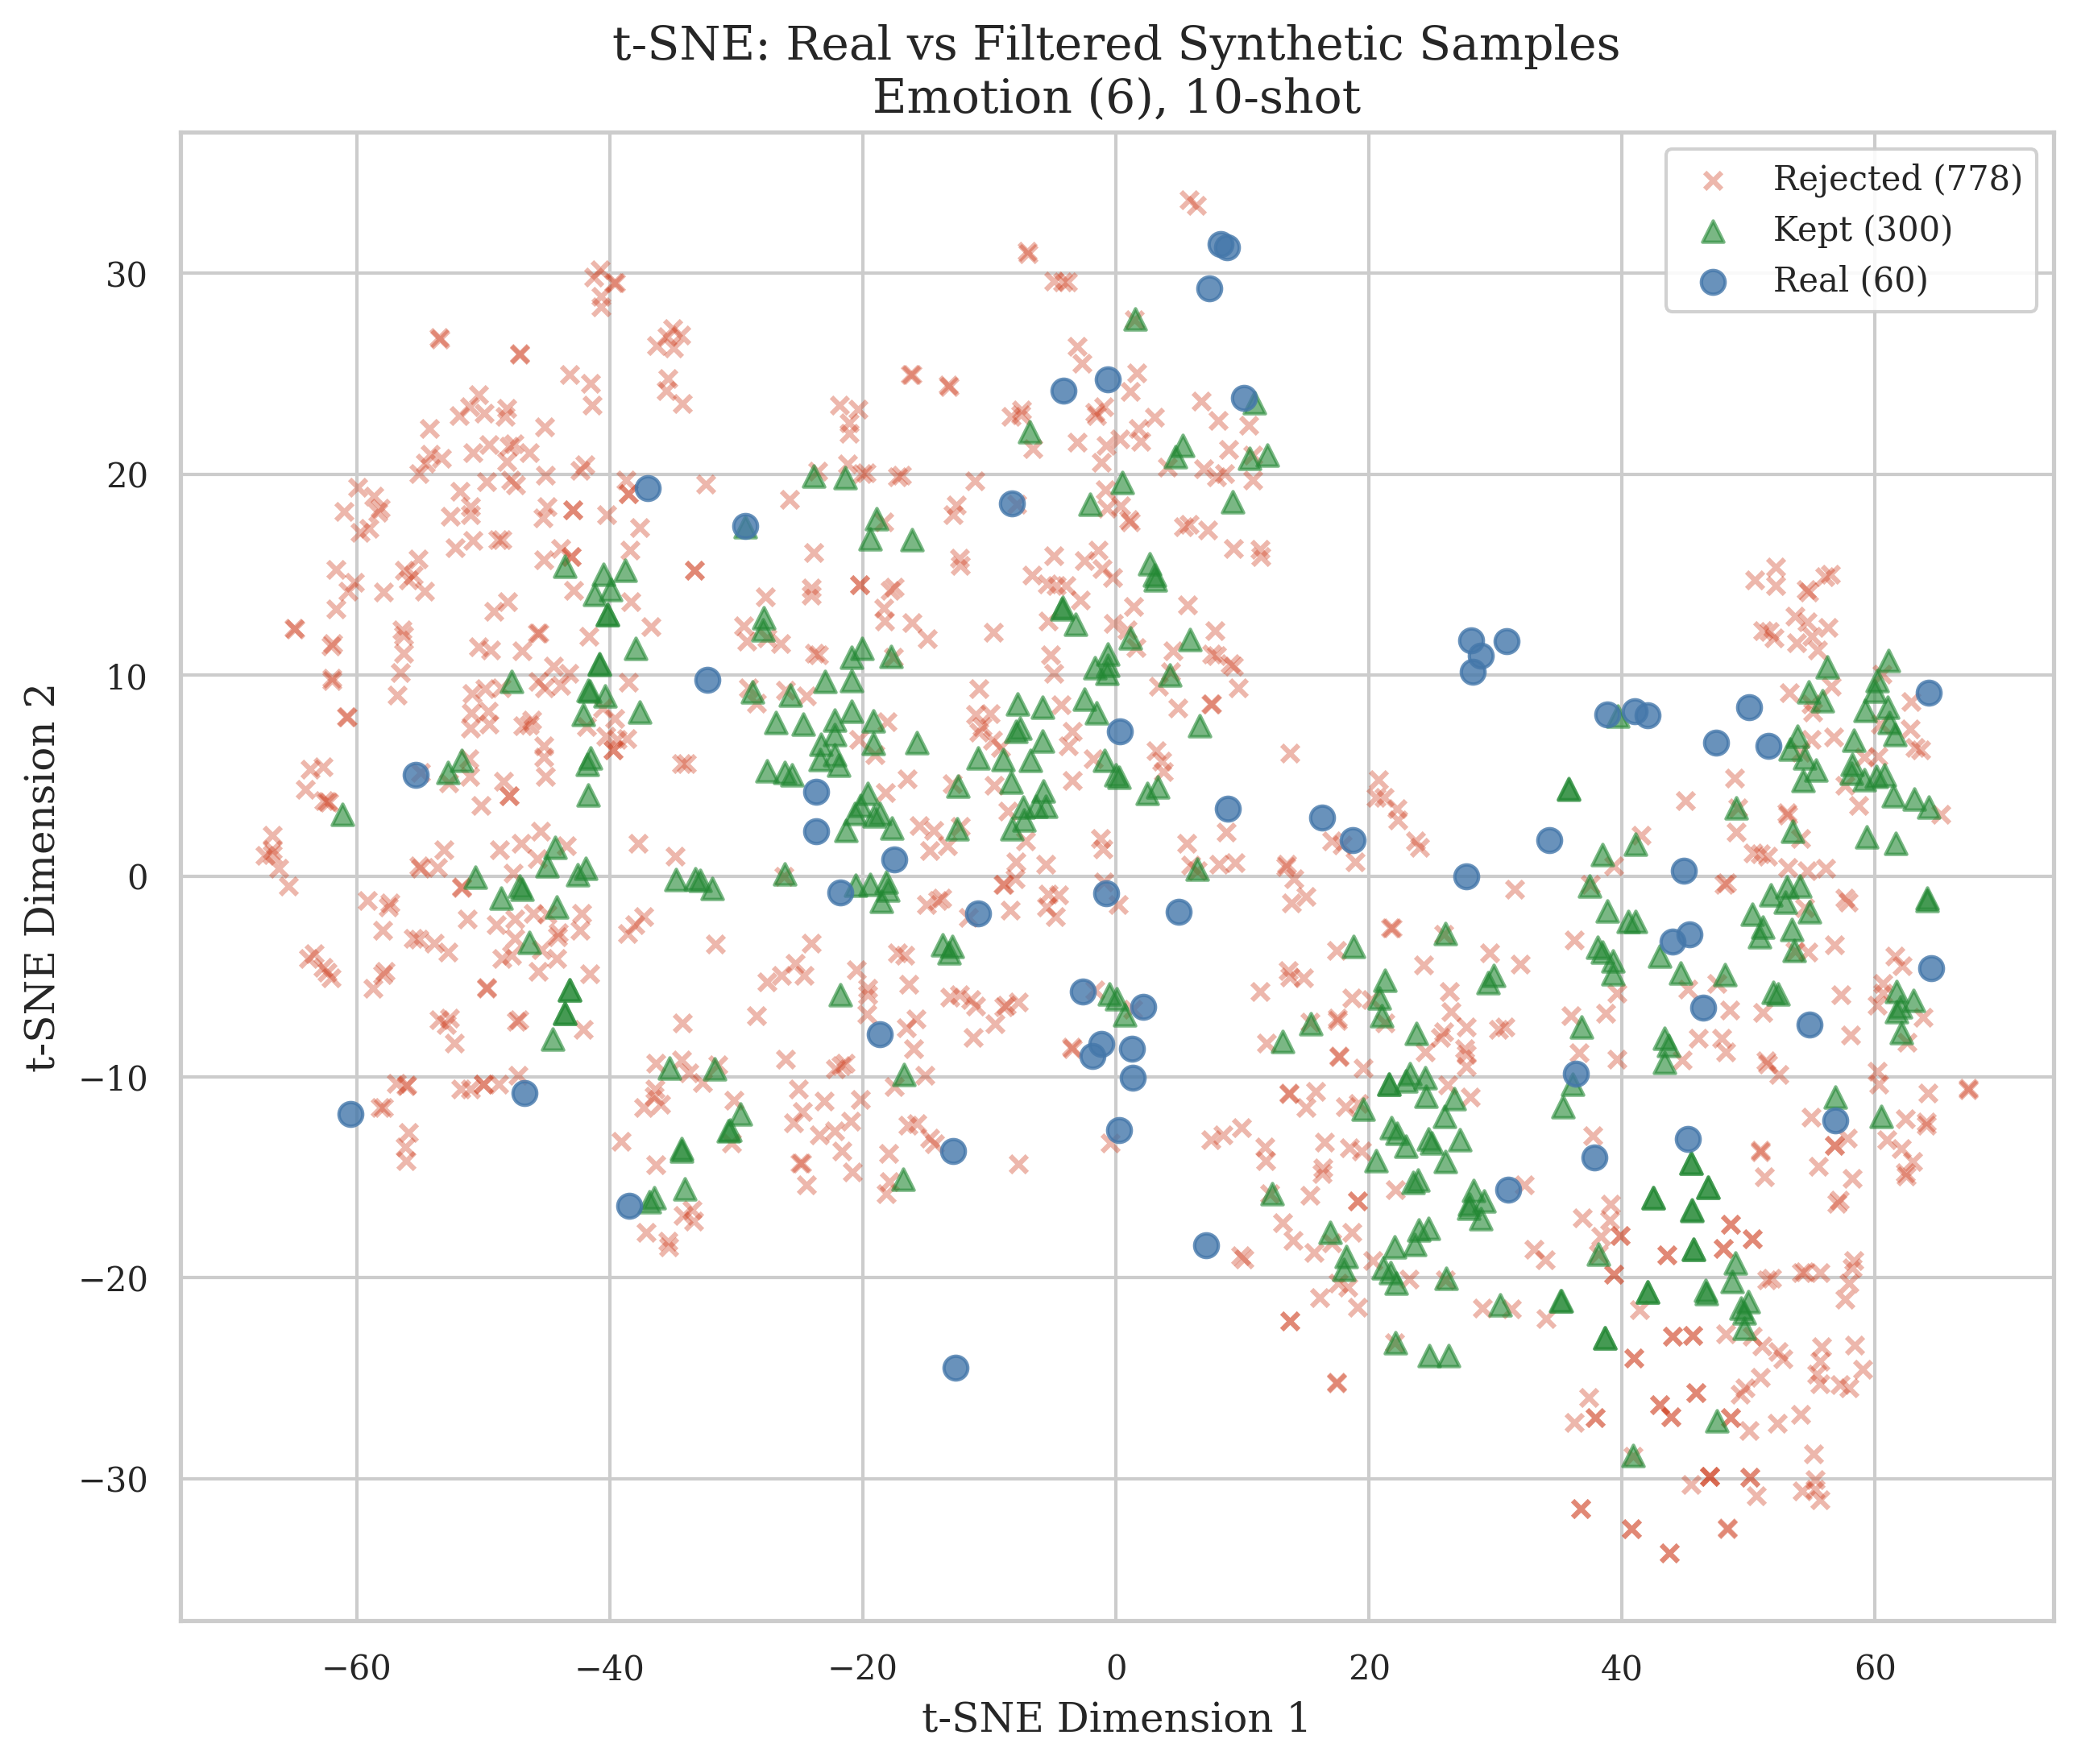
\includegraphics[width=0.85\textwidth]{Figures/fig_tsne_emotion.png}
\caption{Proyección t-SNE para emotion con 10 ejemplos por clase. Las 6 emociones forman conglomerados con diferentes grados de separación. El filtro geométrico selecciona muestras sintéticas que refuerzan los conglomerados existentes sin contaminar regiones de otras clases.}
\label{fig:tsne_emotion}
\end{figure}

\begin{figure}[htbp]
\centering
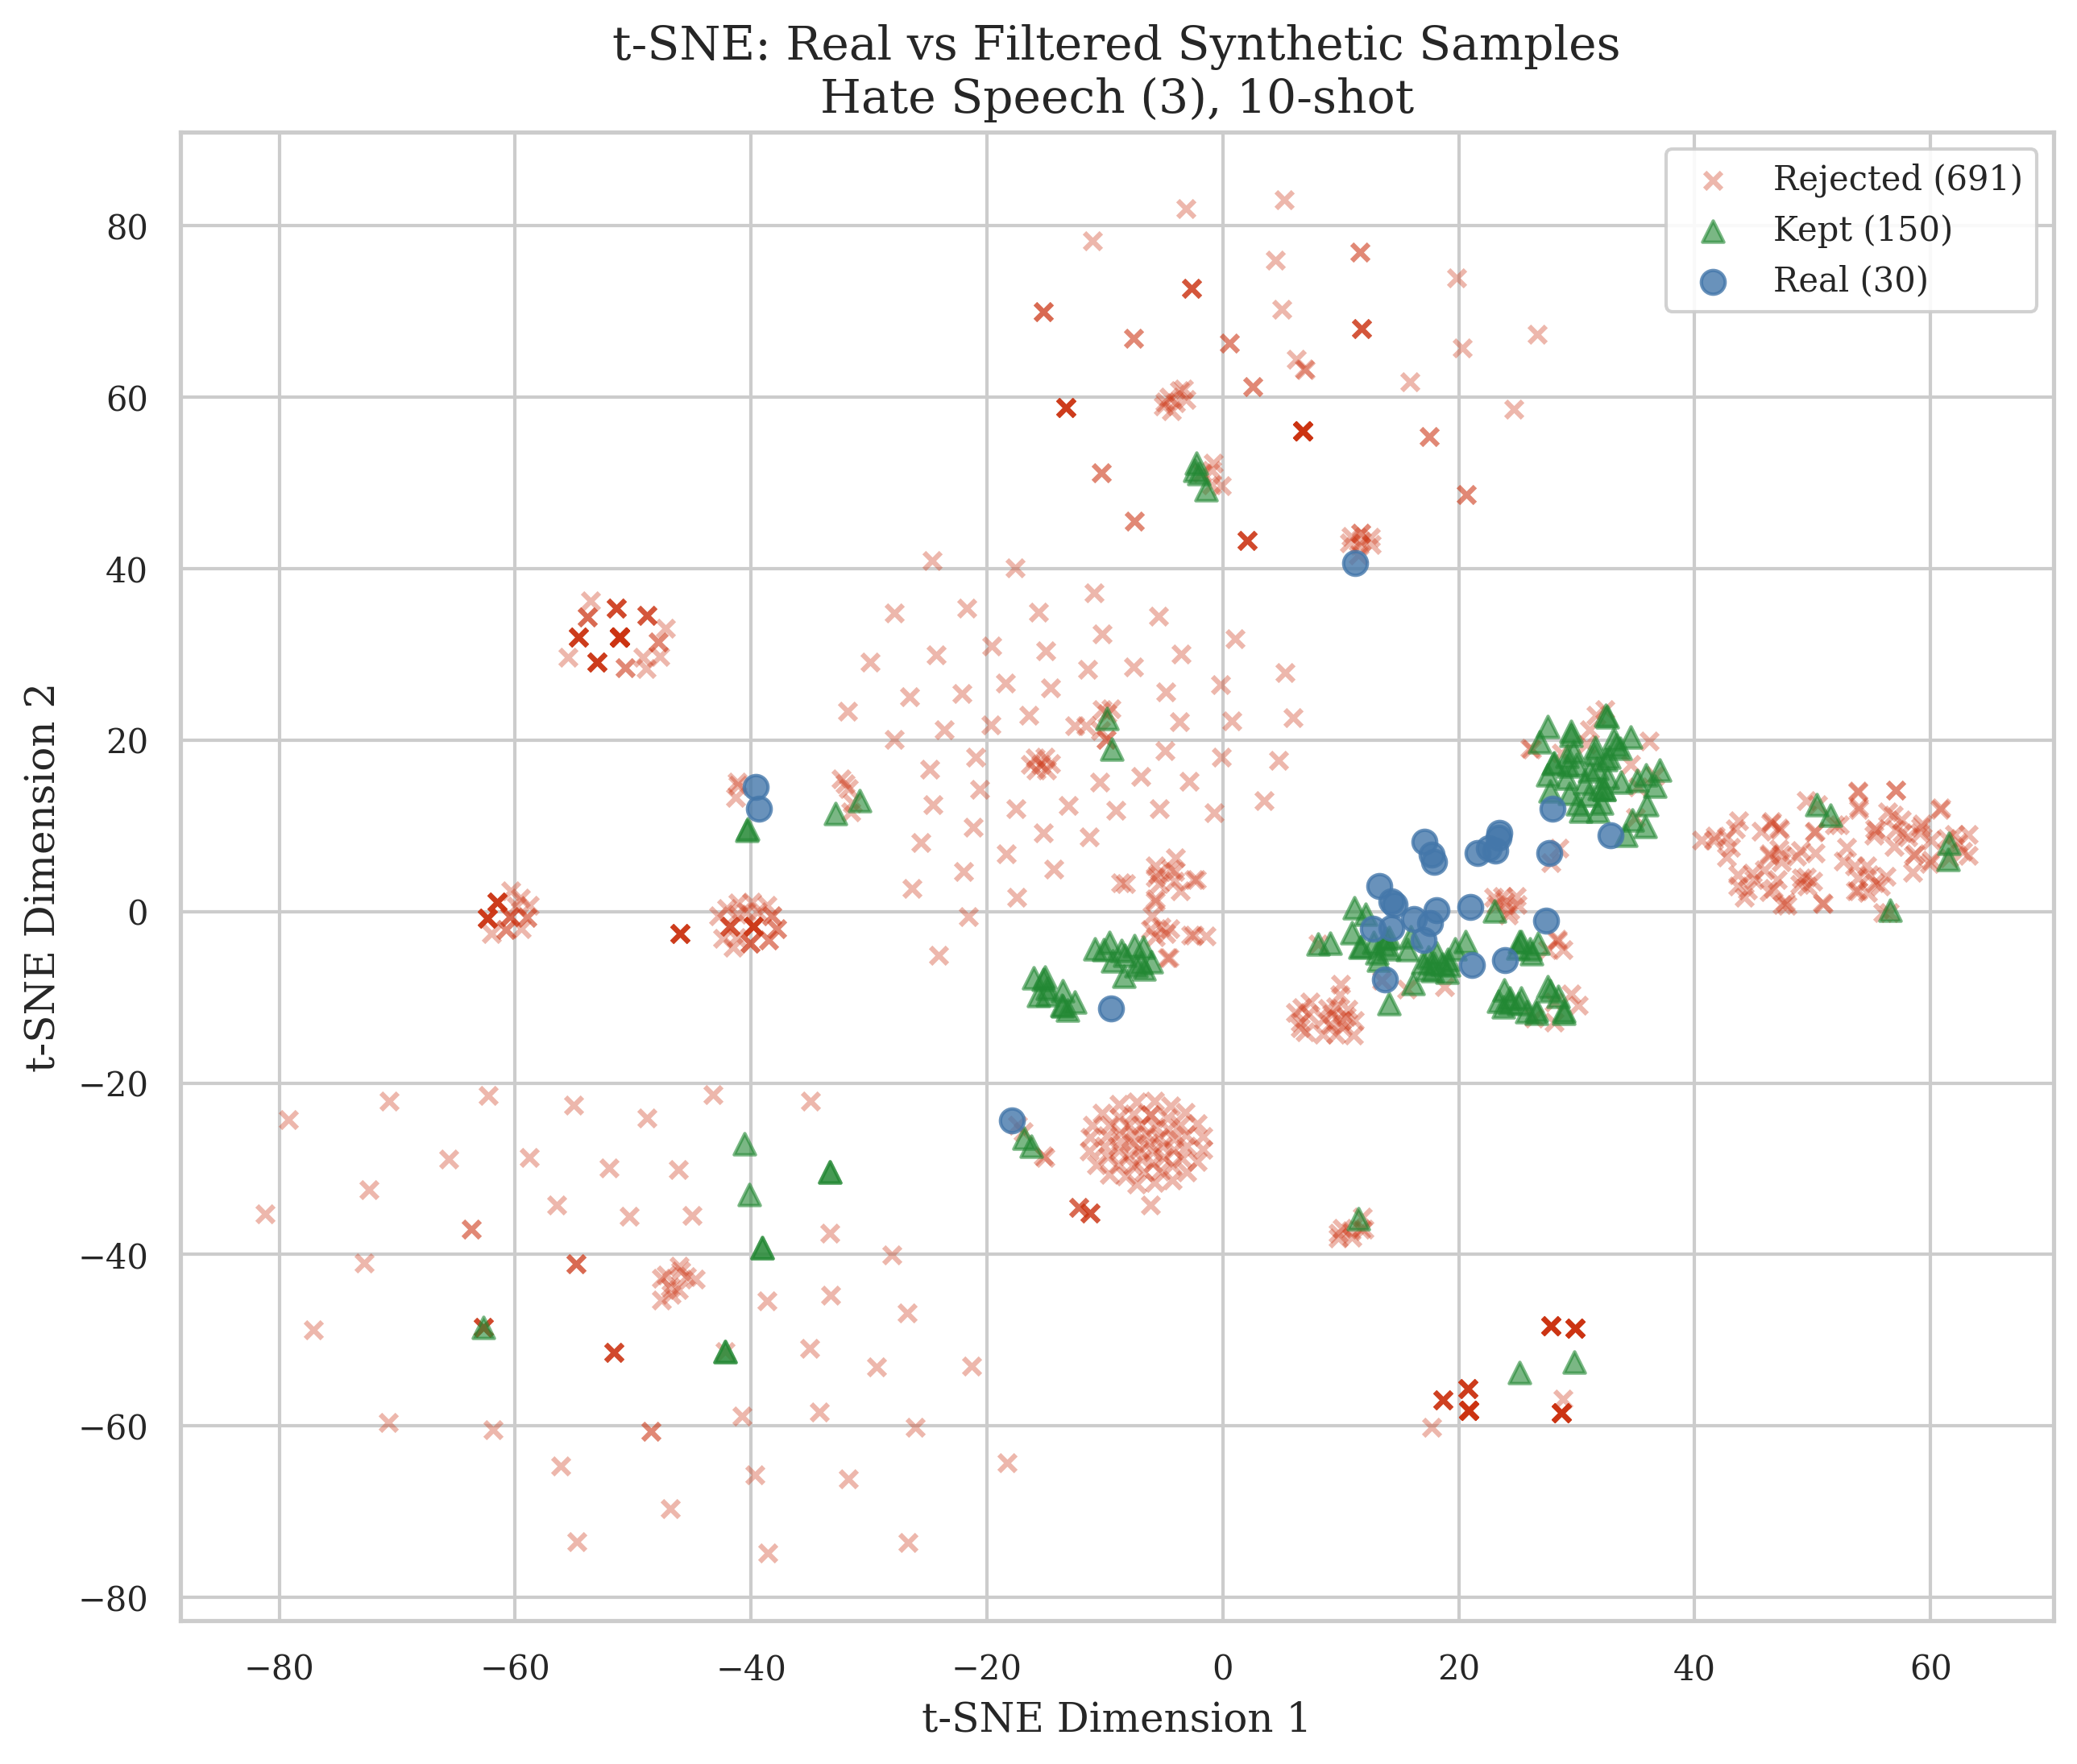
\includegraphics[width=0.85\textwidth]{Figures/fig_tsne_hate_speech.png}
\caption{Proyección t-SNE para hate\_speech\_davidson con 10 ejemplos por clase. Este conjunto presenta mayor solapamiento entre clases. El filtro selecciona preferentemente muestras en regiones donde la clase es dominante, evitando zonas de frontera ambigua.}
\label{fig:tsne_hate_speech}
\end{figure}

Las visualizaciones confirman cualitativamente el mecanismo del filtrado geométrico. Las muestras aceptadas por el filtro se ubican en regiones densas del espacio de embeddings donde la clase es localmente dominante. Las muestras rechazadas tienden a aparecer en 3 patrones: (1) en zonas de frontera entre clases, donde podrían confundir las fronteras de decisión; (2) en regiones periféricas alejadas de la distribución real; y (3) aisladas de cualquier conglomerado, sugiriendo alucinaciones del LLM.

La Figura~\ref{fig:scores_20news} muestra la distribución de puntuaciones del filtro para las muestras aceptadas y rechazadas.

\begin{figure}[htbp]
\centering
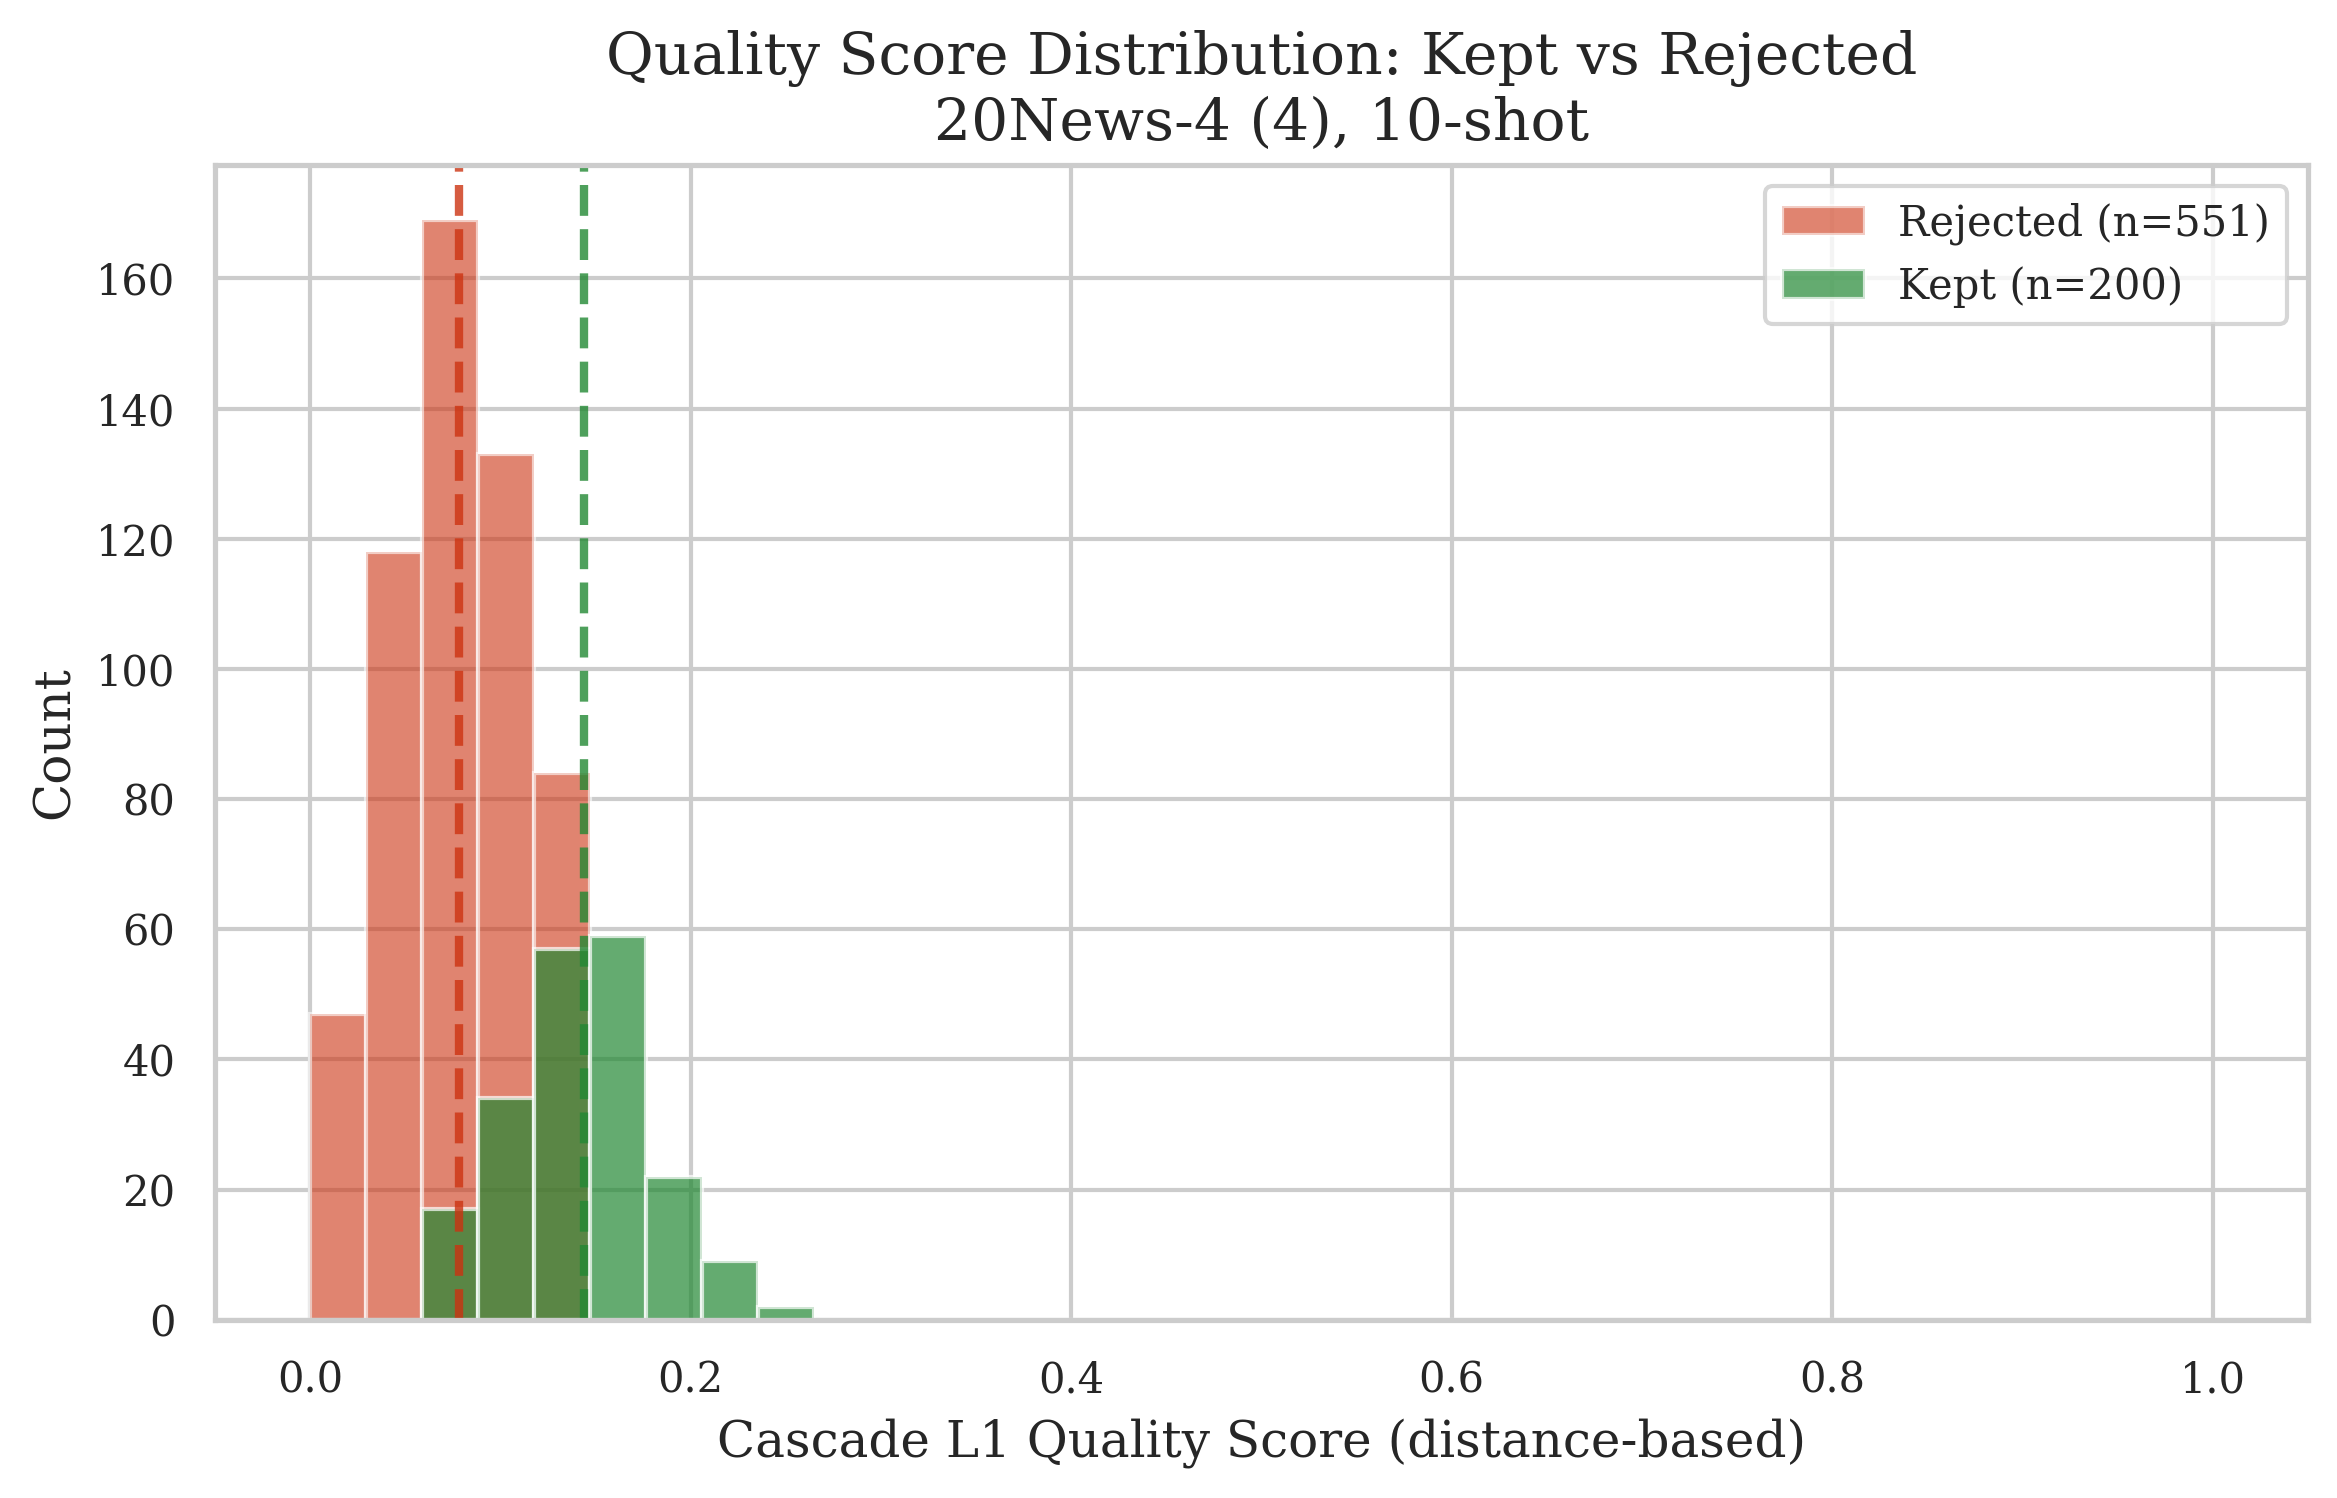
\includegraphics[width=0.85\textwidth]{Figures/fig_scores_20news.png}
\caption{Distribución de puntuaciones del filtro de cascada nivel 1 para 20newsgroups. Las muestras aceptadas (azul) presentan puntuaciones significativamente más altas que las rechazadas (rojo), confirmando la efectividad del criterio de selección basado en distancia.}
\label{fig:scores_20news}
\end{figure}
